\documentclass[a4paper,10pt]{article}
\usepackage[utf8]{inputenc}
\usepackage{graphicx}    
\usepackage{color}
%\usepackage{epsfig}   
\usepackage[font=footnotesize]{subfig}
\usepackage{float}
\usepackage{fancyhdr}                              
\usepackage{makeidx}
\usepackage[nottoc,notlot,notlof]{tocbibind}     
\usepackage{supertabular}
\usepackage{array}              
\usepackage{setspace} 
\usepackage{enumerate}
\usepackage{rotating}
\usepackage{moreverb}
\usepackage{multirow}
\usepackage{amsmath}
\usepackage{amsthm}
\usepackage{amssymb}
\usepackage{captcont}
\usepackage{verbatim}
\usepackage{titlesec}
\usepackage{url}
\usepackage{hyperref}
\usepackage{lipsum}
\usepackage{tikz}
\usepackage{pgf-pie}
\usepackage{pgfplots}
\usepackage{array}
\usepackage{booktabs}
\usepackage{blindtext}
\usepackage{tabularx}
\usepackage{pbox}
%\usepackage[utf8]{inputenc}
\usepackage{commath}

\newcolumntype{L}[1]{>{\raggedright\let\newline\\\arraybackslash\hspace{0pt}}m{#1}}
\usepackage[margin=1in]{geometry}
\begin{document}


\section{Analysis of Methods implemented}

The library has 5 methods to detect anomalies.
Following table describes the method and limitations of every method:


\begin{table}[H]
\centering
\resizebox{\textwidth}{!}{
\begin{tabular}{|L{3cm} | L{5cm} | L{8cm}|}
\hline                                                                                                                                                                                                                                                                                                                                                  
Window Correlation                    & Detects if the two timeseries follows their expected behaviour or not. i.e if the two timeseries are expected to move in tandem then it reports the tenures where they don't move in tandem and vice- versa                                                            & \begin{itemize}
                                                                                                                                                                                                                                                                                                              \item Result of method depends on window size. So if the anomaly occurred for very small time, it won't be reported. (See Figure \ref{fig:20110106_0108})
                                                                                                                                                                                                                                                                                                              \item Reports results even though the fluctutaions are not very prominent. (See Figure \ref{fig:20080306_0320}) the deviation in prices were not huge but incident was reported because the two timeseries moved out of tandem.
                                                                                                                                                                                                                                                                                                              \item Result is also dependant on selected threshold.
                                                                                                                                                                                                                                                                                                              \end{itemize}
 \\ \hline
Slope-Based Method                    & Reports incidents when one timeseries change its value faster than other.Window correlation miss the incidents when one timeseries changes its values faster than other since it just focus on the direction of change and not on rate of change. (See Figure \ref{fig:12111})     & \begin{itemize}
                                                                                                                                                                                                                                                                                                                  \item Result of method depends on window size. So if the anomaly occurred for very small time, it won't be reported.
                                                                                                                                                                                                                                                                                                                  \item Since it only checks rate of change in timeseries, it reports cases when retail prices decline to great rate than others which is ideally a good case. (See Figure \ref{fig:12112})
                                                                                                                                                                                                                                                                                                                  \item Result is also dependant on selected threshold. (See Figure \ref{fig:12113})
                                                                                                                                                                                                                                                                                                                 \end{itemize}
 \\ \hline
Linear Regression                     & It tries to build a linear model between two timeseries. Reports all the points which deviates much from the predicted value.                                                                                                                                          & \begin{itemize}
                                                                                                                                                                                                                                                                                                                  \item Efficiency of method depends on to what extent two timeseries are linearly dependant.
                                                                                                                                                                                                                                                                                                                  \item Result is dependant on selected threshold.                                                                                                                                                                                                                                                        
                                                                                                                                                                                                                                                                                                                 \end{itemize}
  \\ \hline
Multivarite- timeseries               & It also builds a vector- autoregressive model based on multiple timeseries which affect each others value.Reports all the dates which tends to deviate too much from the predicted value. Considers trend and seasonality component of timeseries..(See Figure \ref{fig:20130719_0911}) & \begin{itemize}
                                                                                                                                                                                                                                                                                                                  \item Result is dependant on selected threshold.
                                                                                                                                                                                                                                                                                                                 \end{itemize}                                                                                                                                                                                                                                                                                                                                                \\ \hline
Graph Based                           & It considers trend and seasonality in the timeseries while building model. Reports all the dates which seems deviating much from the past data.(See Figure \ref{fig:12331})                                                                                                     & \begin{itemize}
                                                                                                                                                                                                                                                                                                                  \item Result is dependant on number of anomalous points selected. 
                                                                                                                                                                                                                                                                                                                 \end{itemize}                                                                                                                                                                                                                                                                                                                              \\ \hline
	\end{tabular}}
	\caption{Description on methods}
	\label{table:MethodDescription}
\end{table}

\begin{figure}[H]
\centering
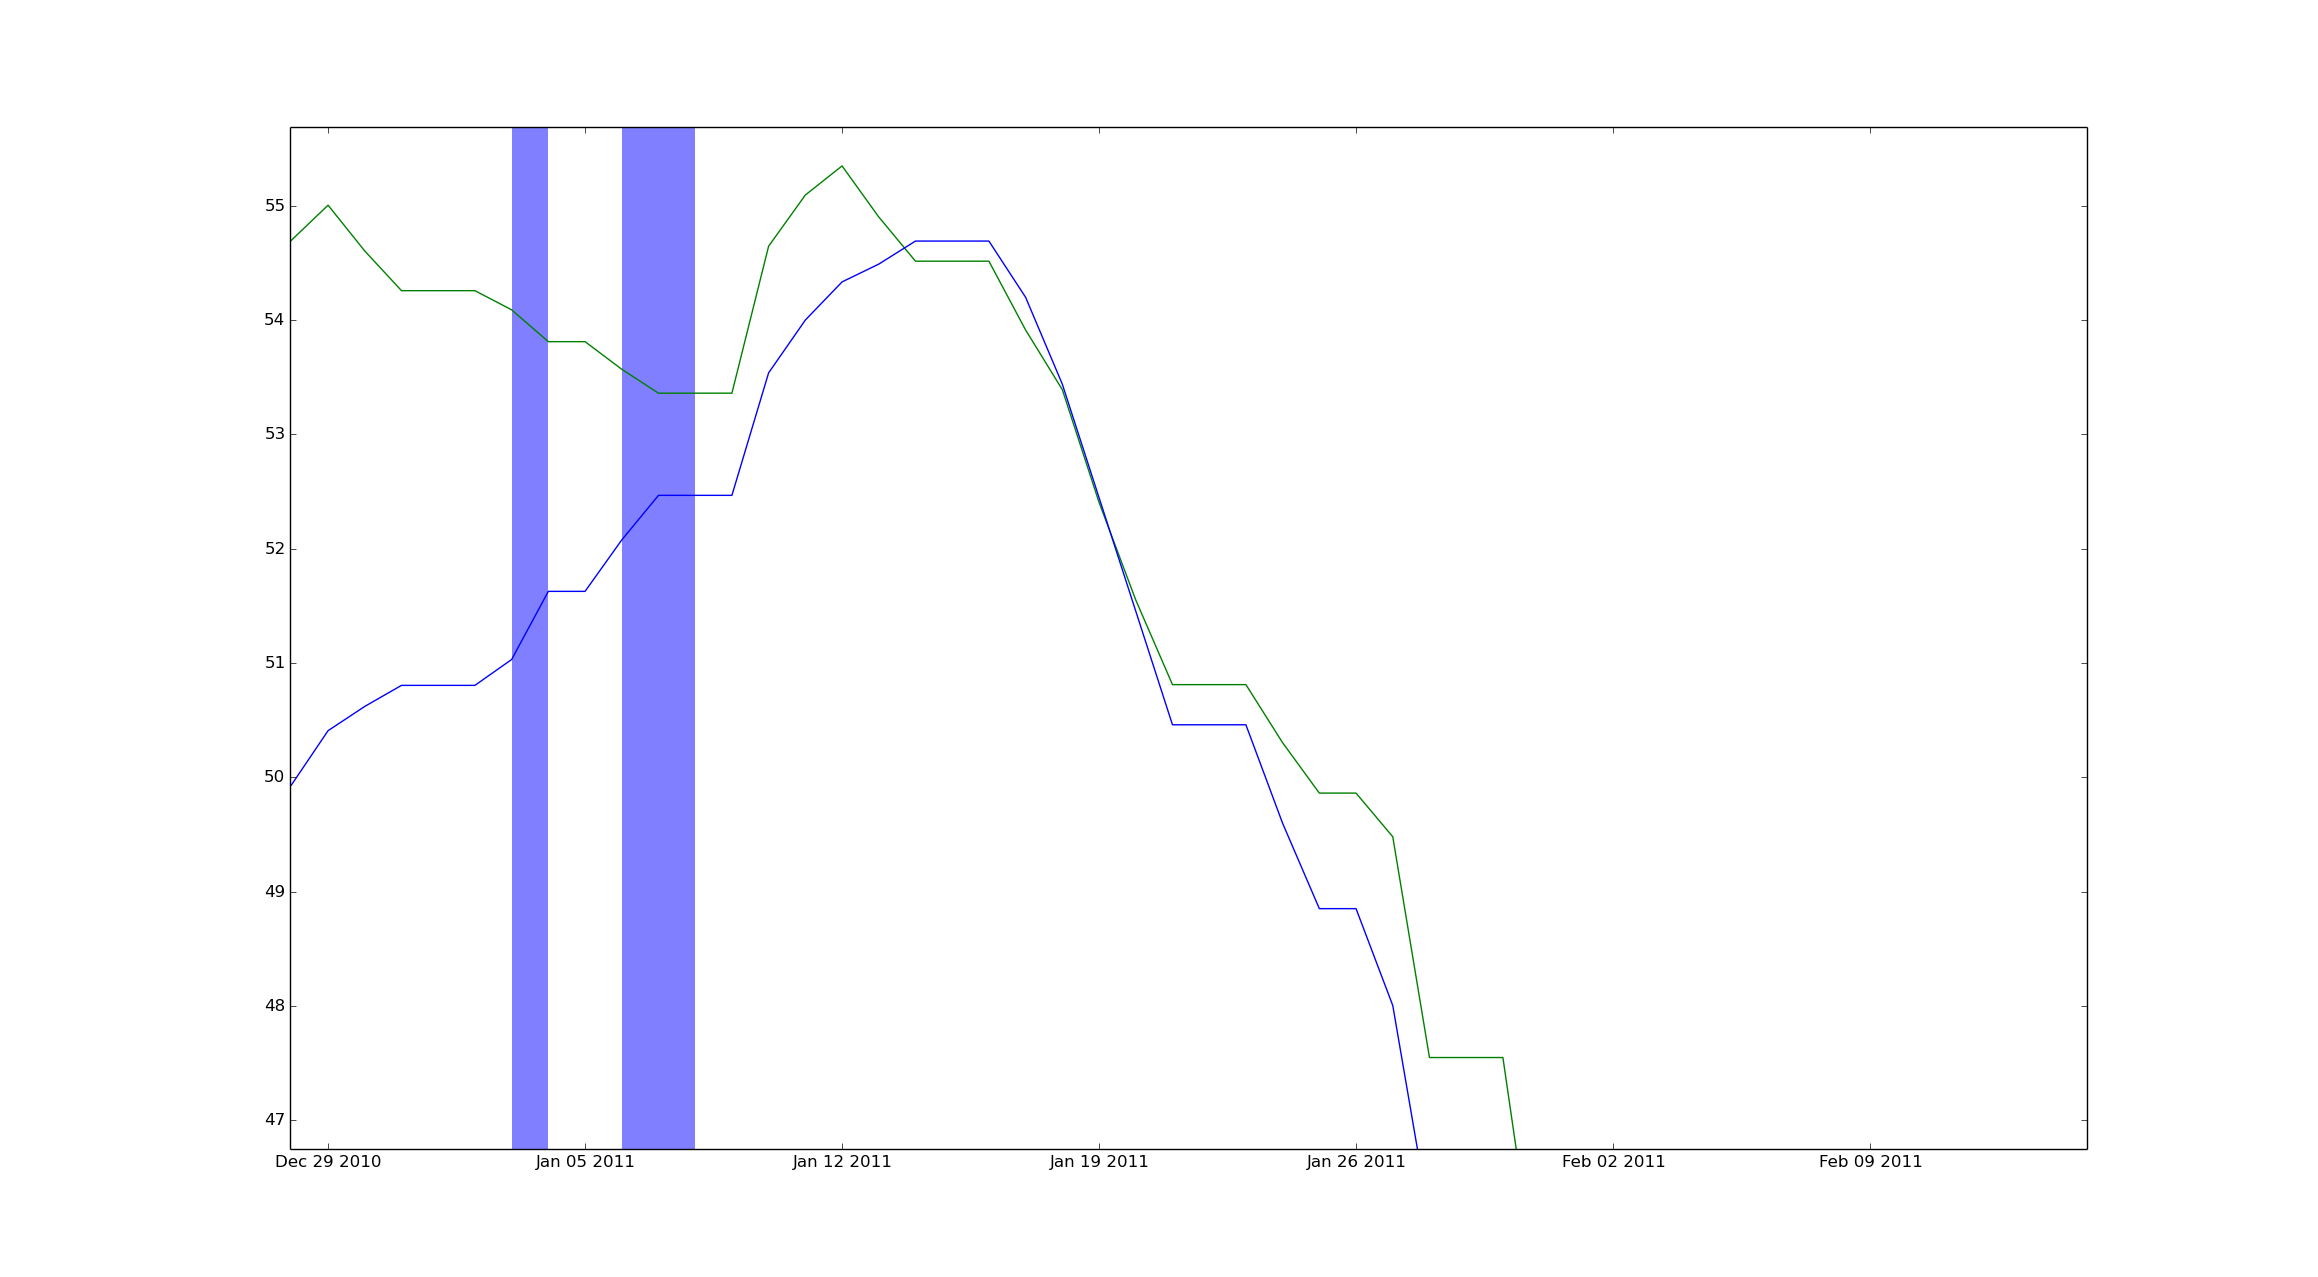
\includegraphics[width=0.8\textwidth]{graphs/20110106_0108.png}
\caption{Window based correlation (Green line - Centre Retail Price, Blue Line - Average Retail Price)}
\label{fig:20110106_0108}
\end{figure}

\begin{figure}[H]
\centering
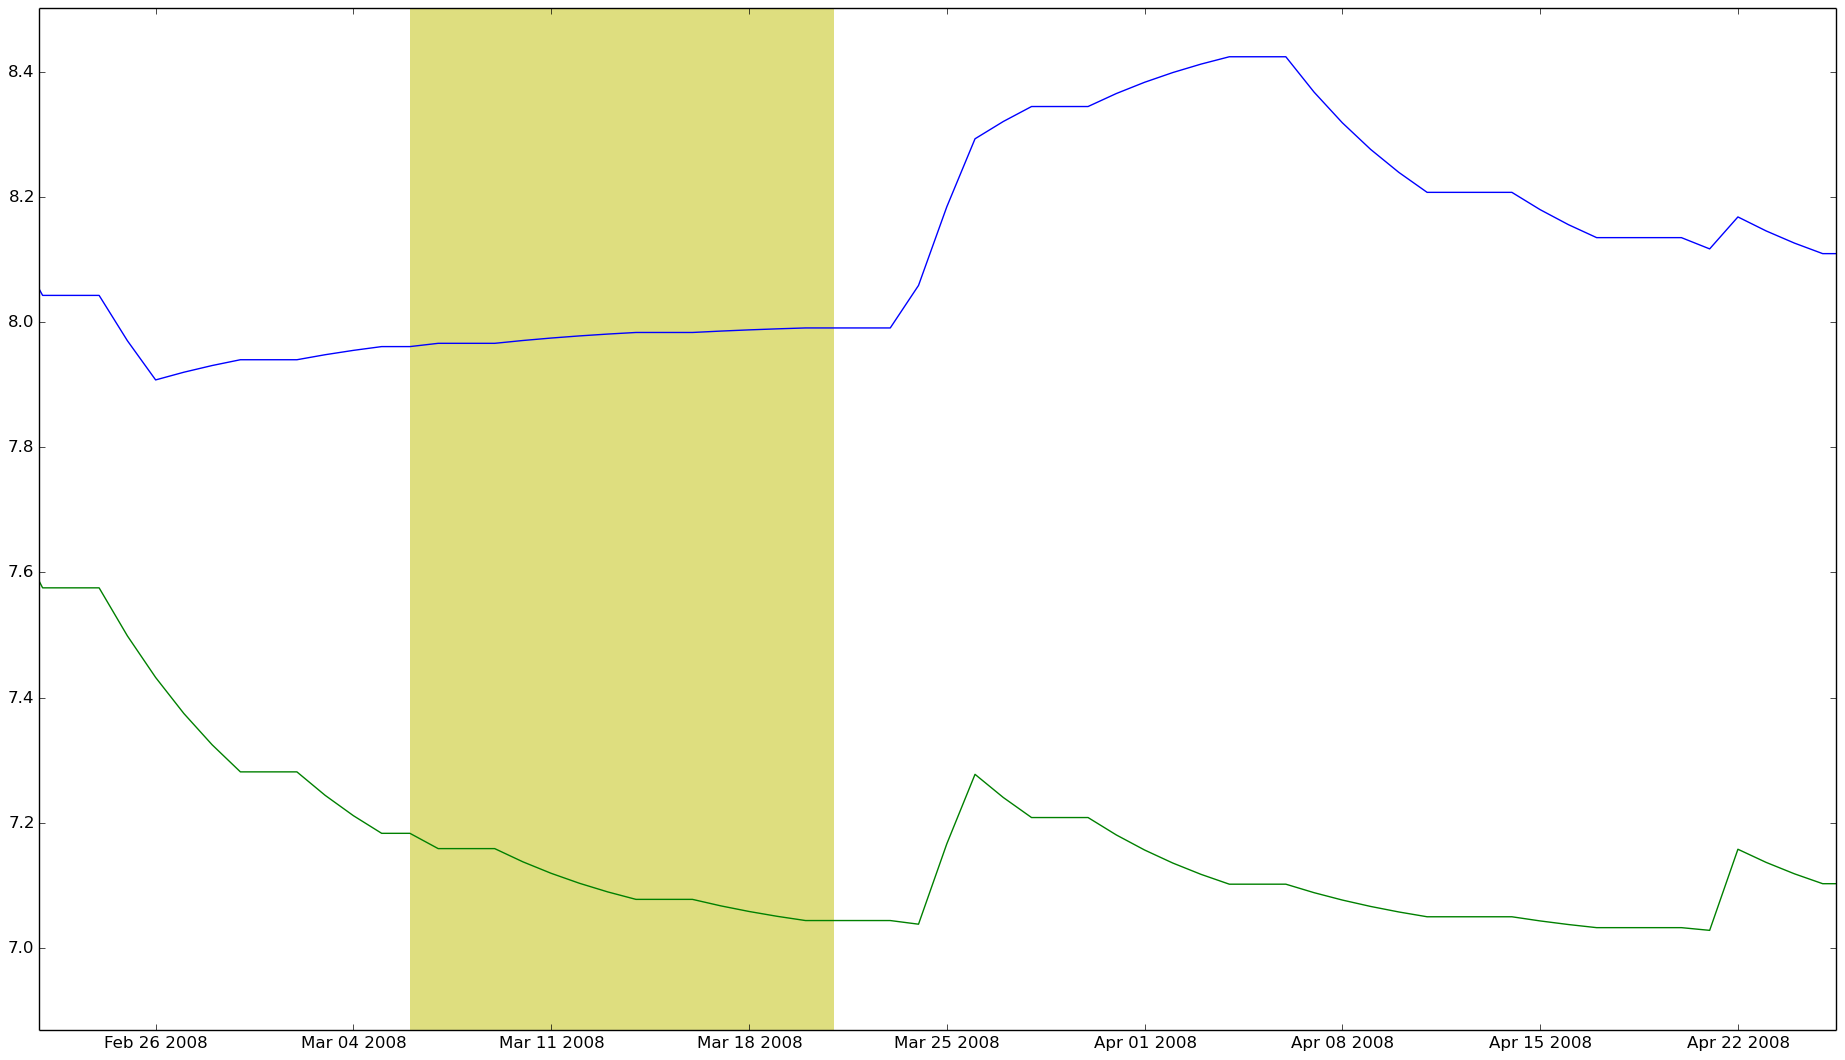
\includegraphics[width=0.8\textwidth]{graphs/20080306_0320.png}
\caption{Window based correlation (Green line - Centre Retail Price, Blue Line - Average Retail Price)}
\label{fig:20080306_0320}
\end{figure}

\begin{figure}[H]
\centering
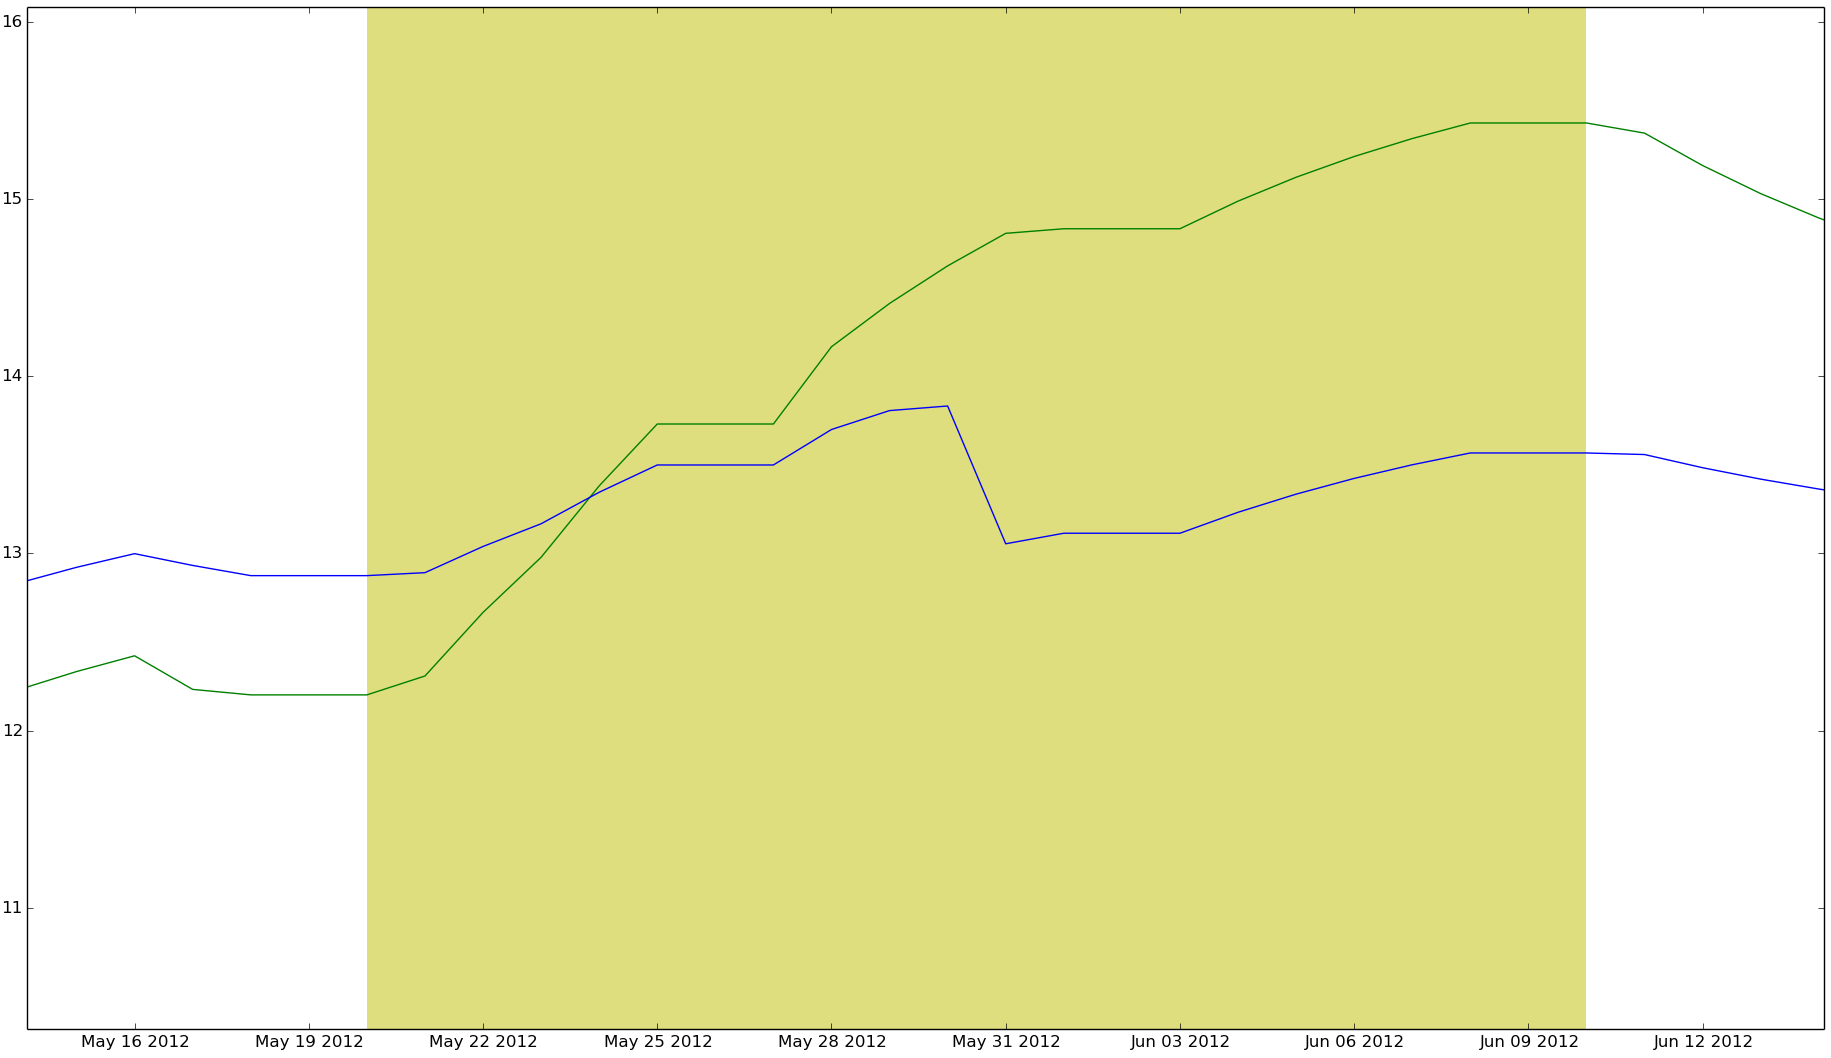
\includegraphics[width=0.8\textwidth]{graphs/12111.png}
\caption{Slope Based Anomaly Detection (Green line - Centre Retail Price, Blue Line - Average Retail Price)}
\label{fig:12111}
\end{figure}

\begin{figure}[H]
\centering
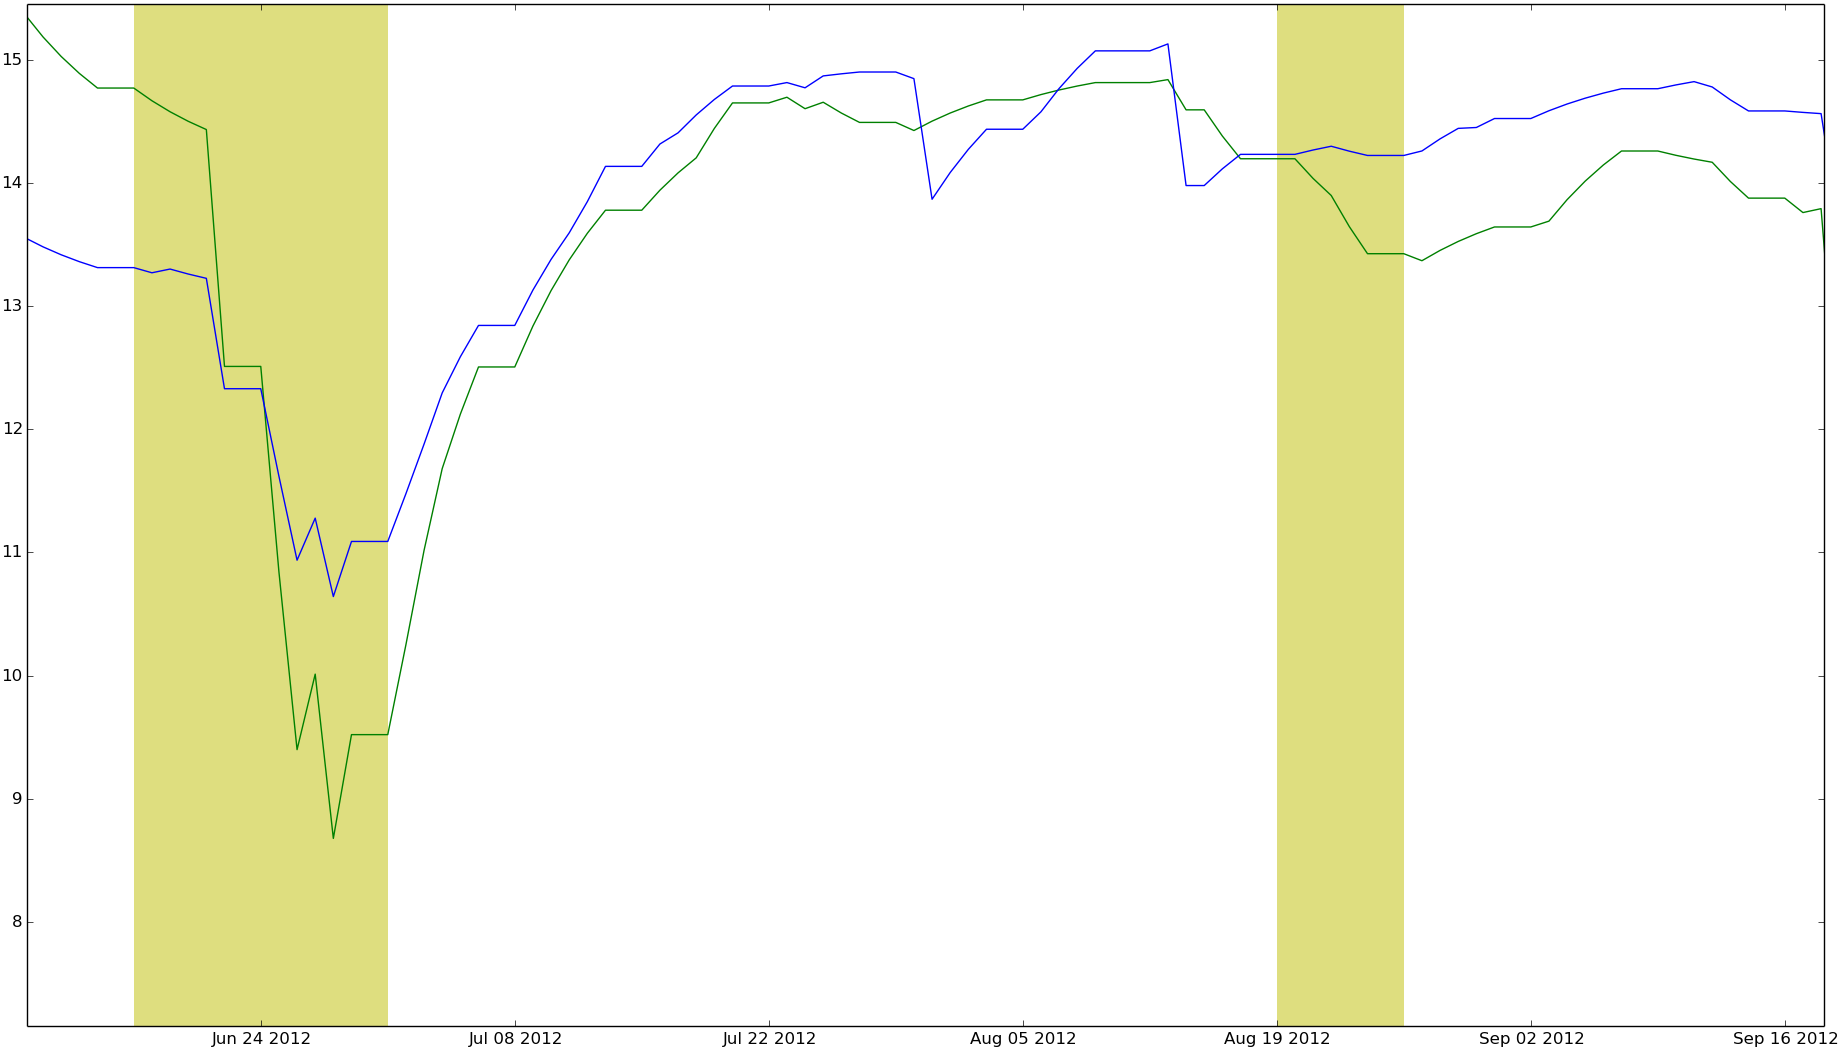
\includegraphics[width=0.8\textwidth]{graphs/12112.png}
\caption{Slope Based Anomaly Detection (Green line - Centre Retail Price, Blue Line - Average Retail Price)}
\label{fig:12112}
\end{figure}

\begin{figure}[H]
\centering
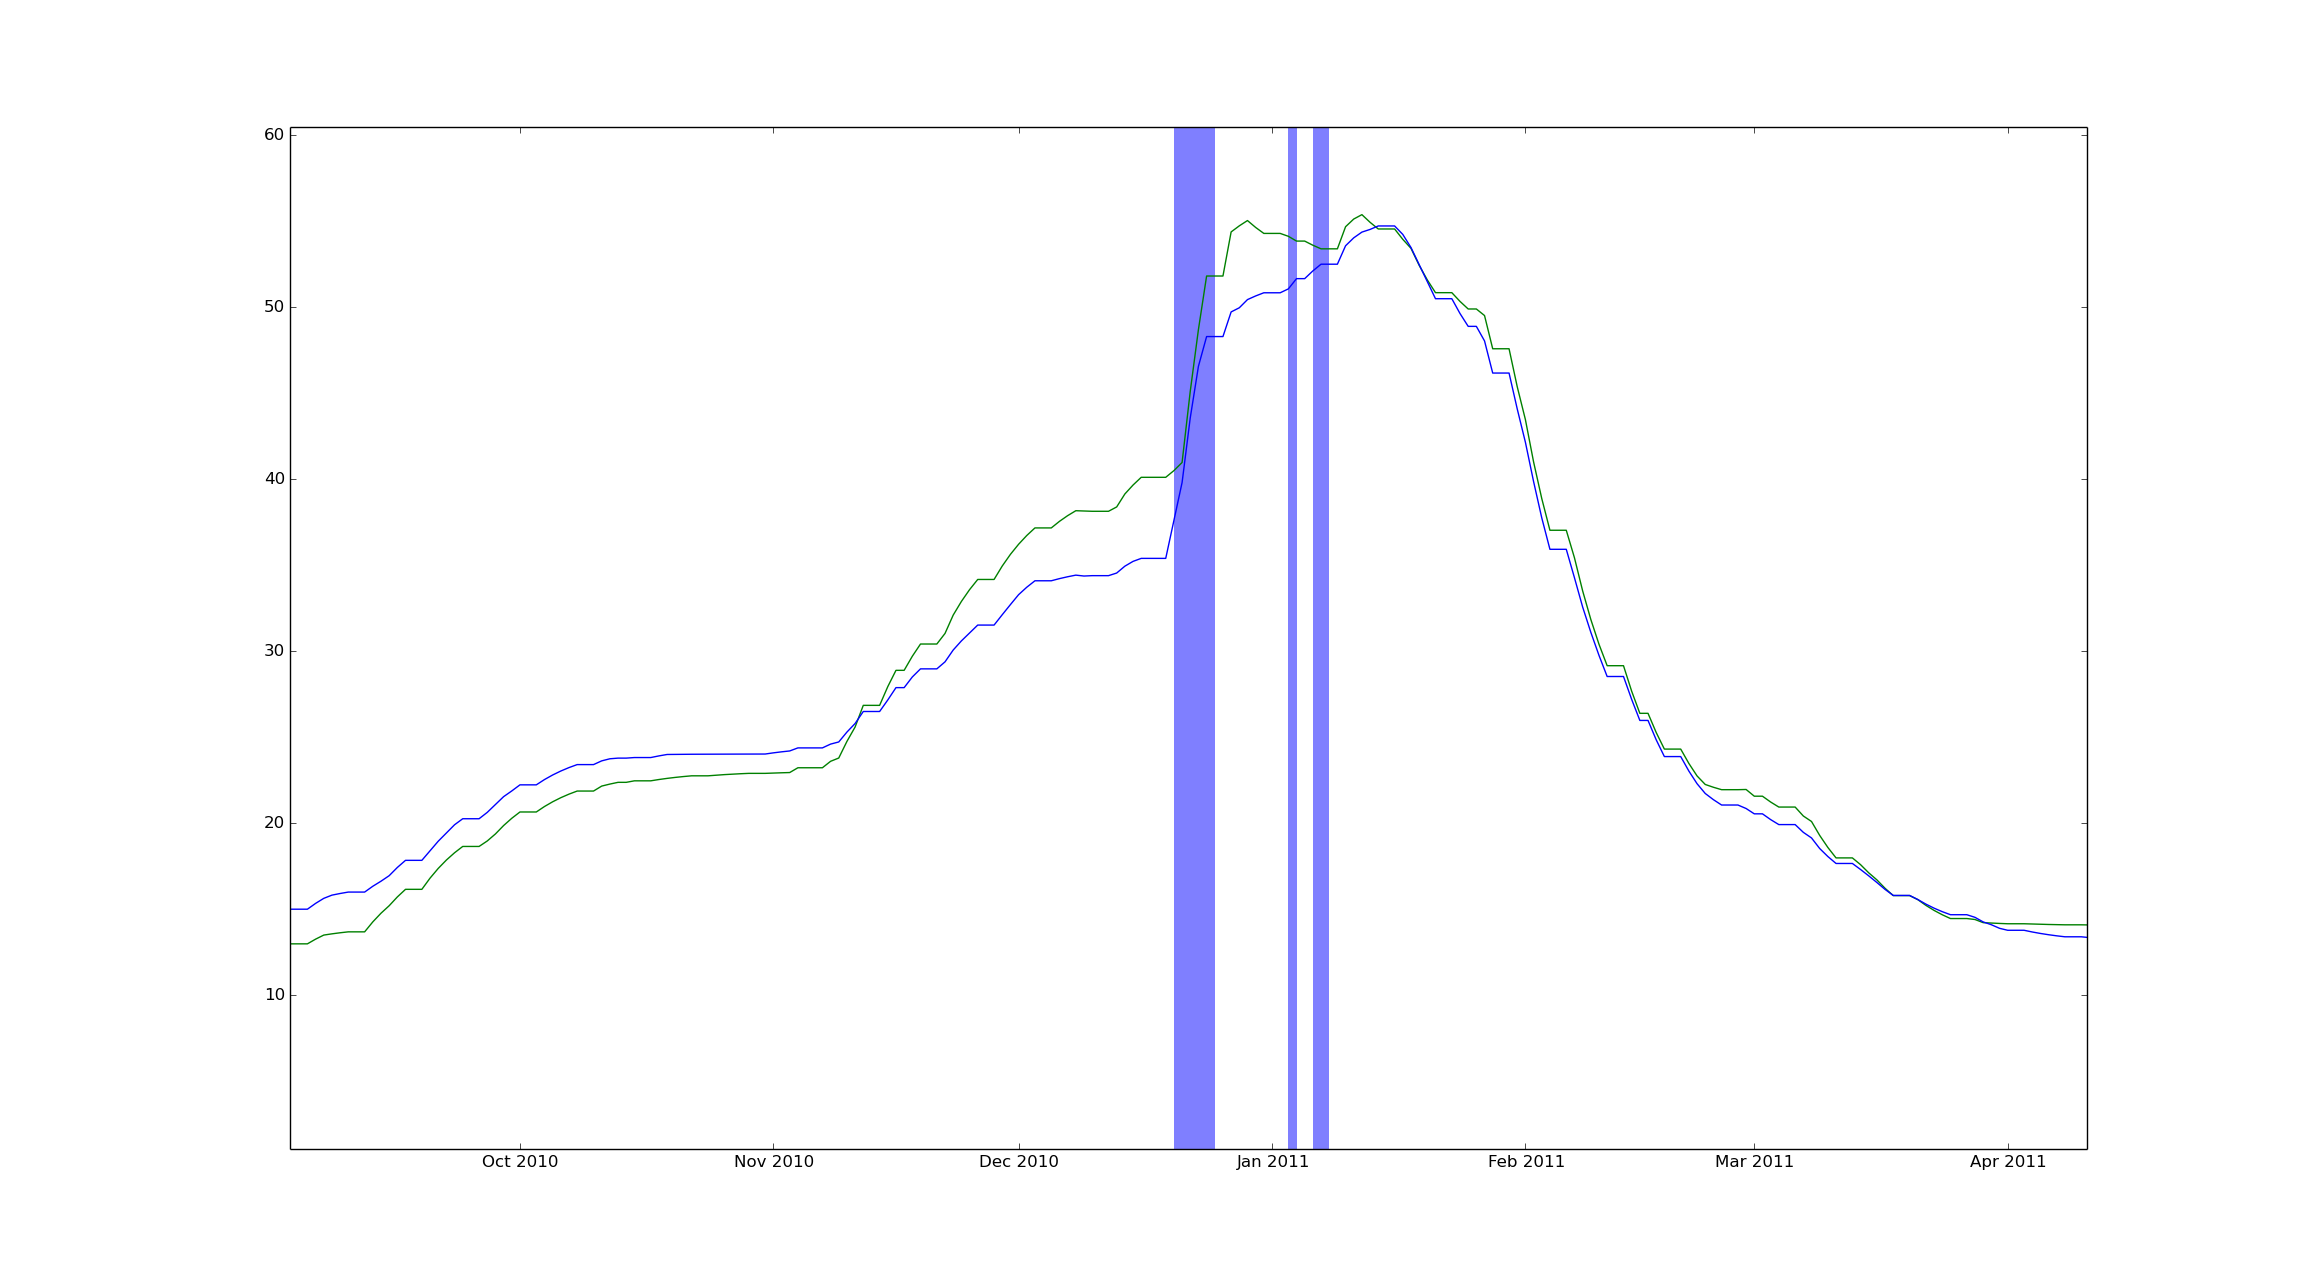
\includegraphics[width=0.8\textwidth]{graphs/12113.png}
\caption{Slope Based Anomaly Detection (Green line - Centre Retail Price, Blue Line - Average Retail Price)}
\label{fig:12113}
\end{figure}

\begin{figure}[H]
\centering
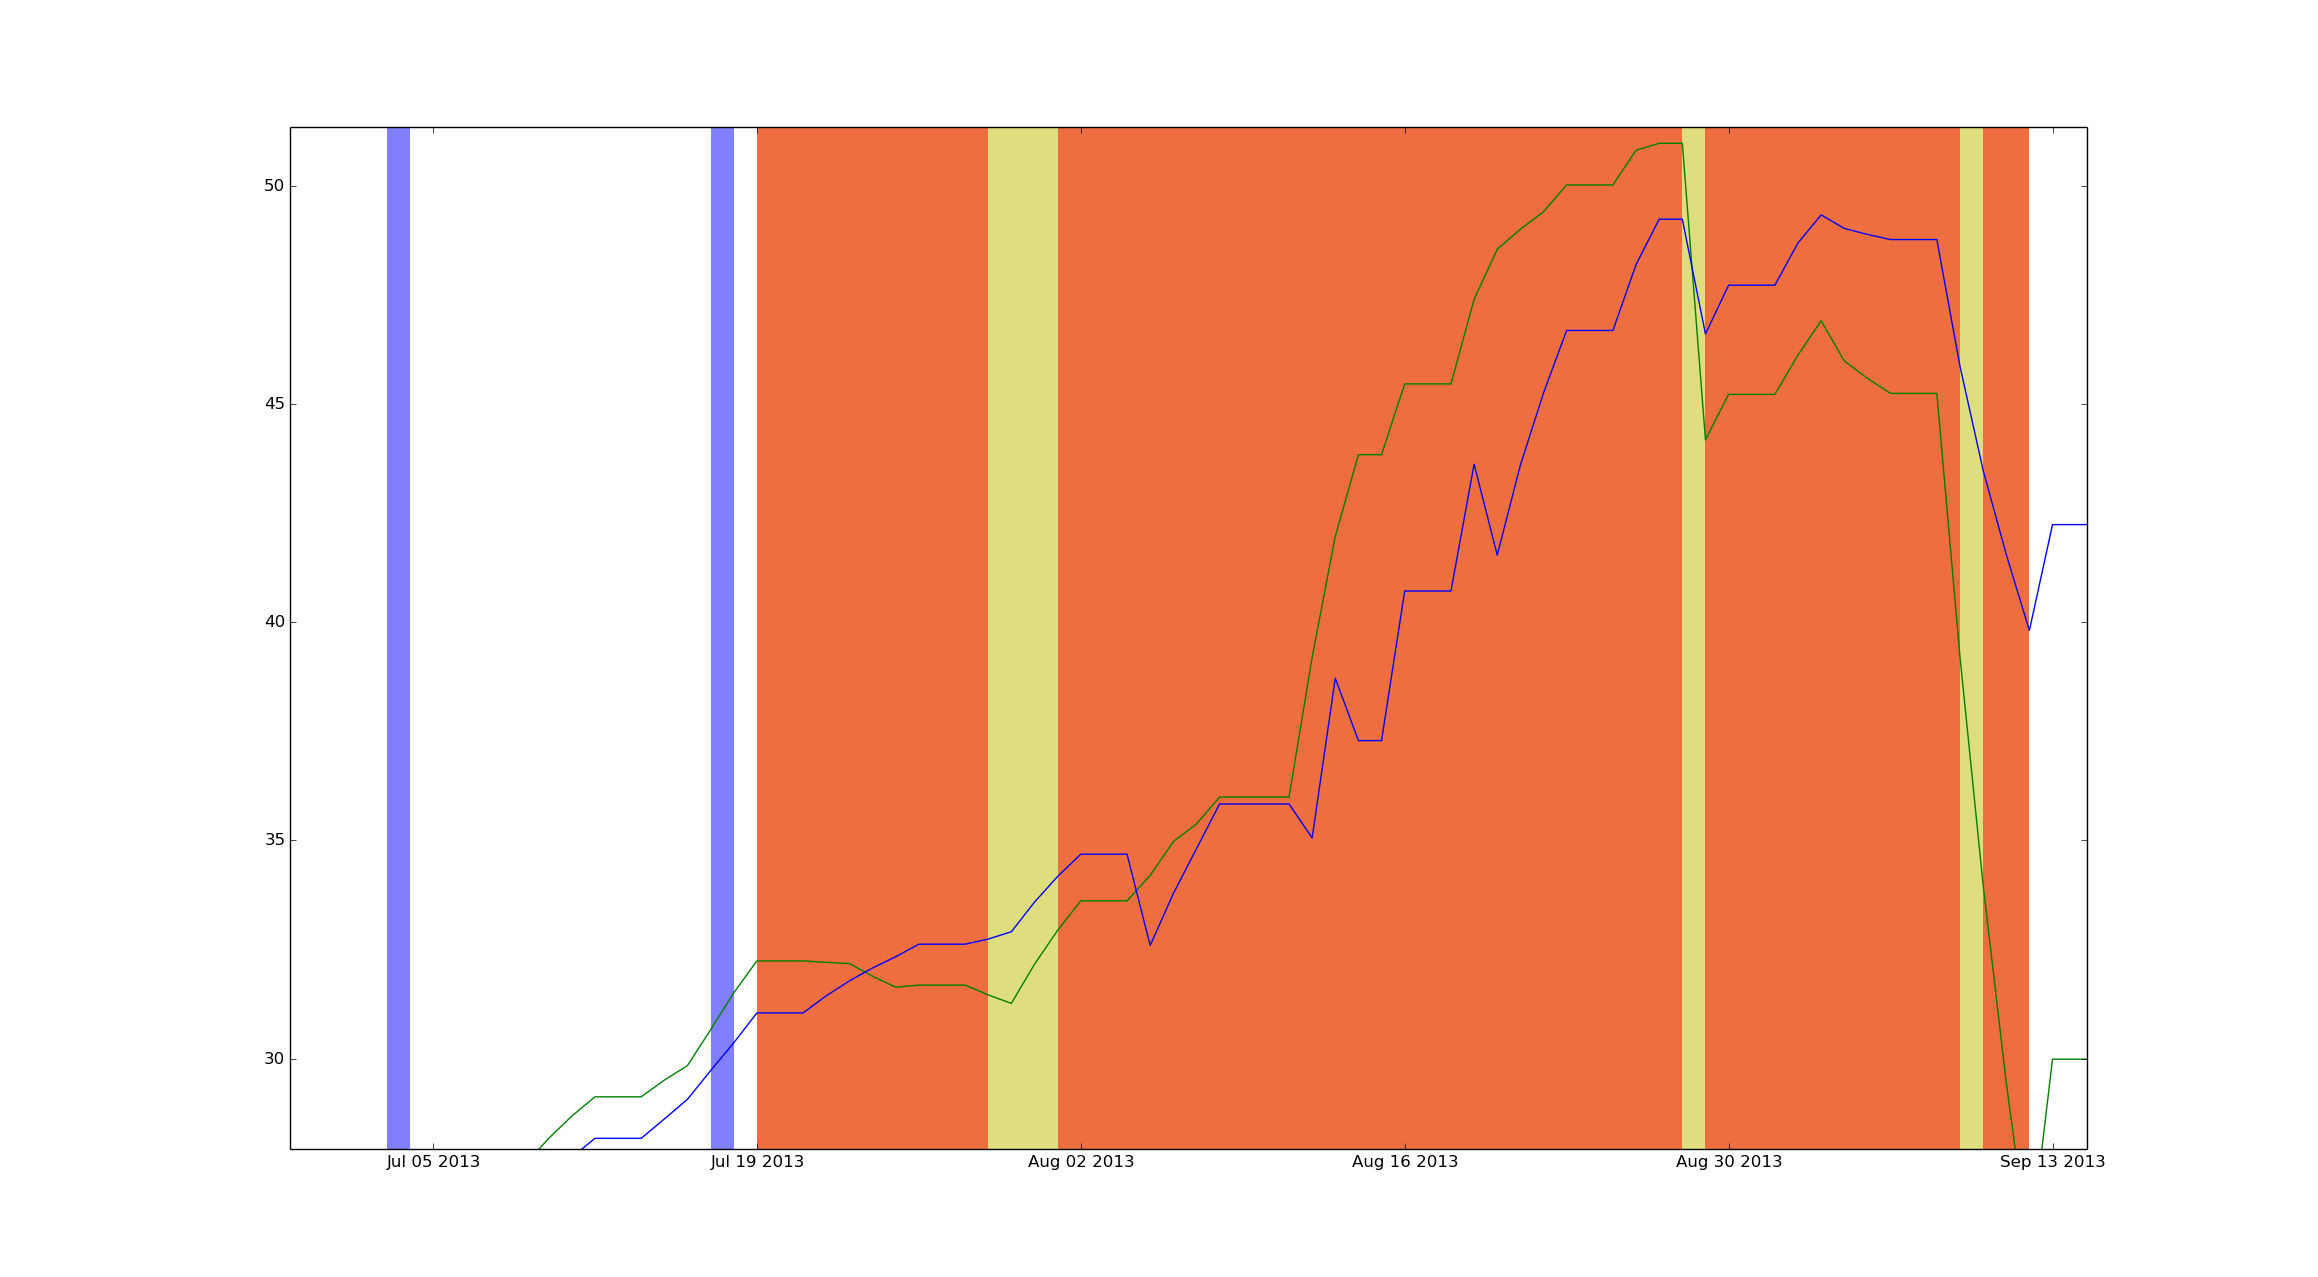
\includegraphics[width=0.8\textwidth]{graphs/20130719_0911.png}
\caption{Vector Autoregressive (Green line - Centre Retail Price, Blue Line - Average Retail Price)}
\label{fig:20130719_0911}
\end{figure}

\begin{figure}[H]
\centering
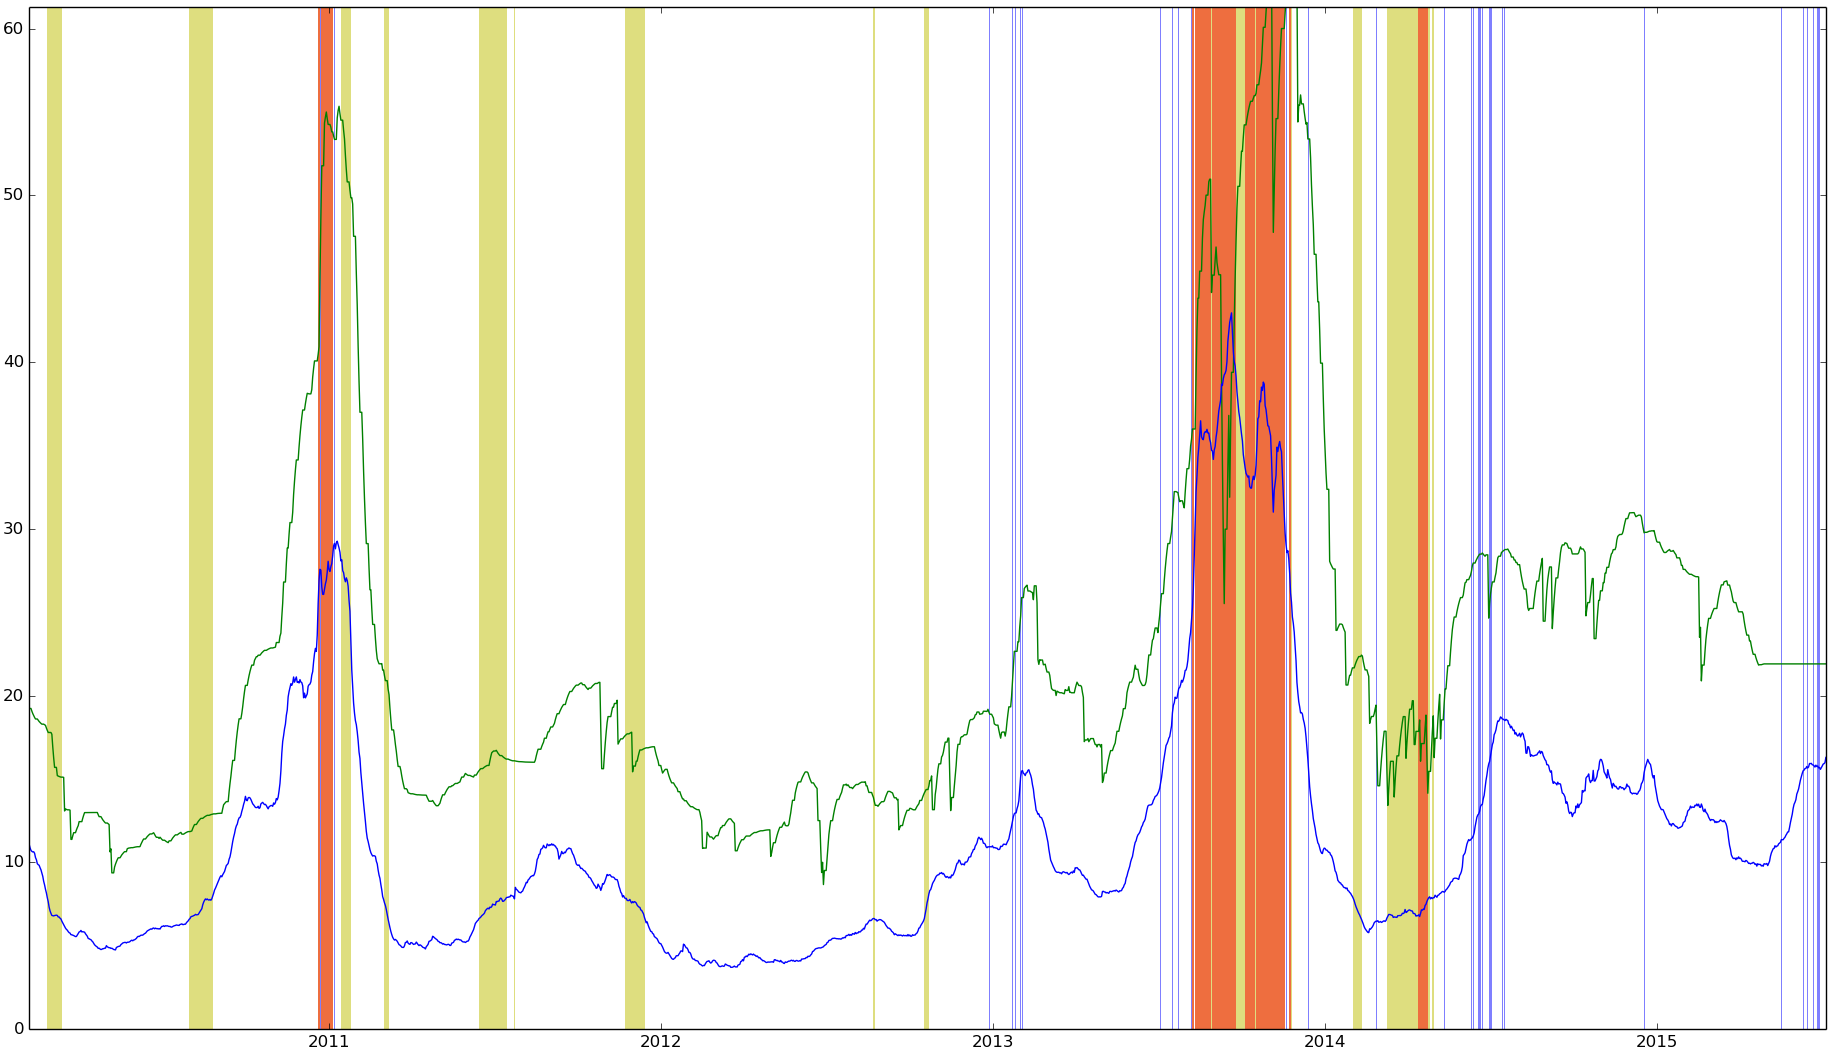
\includegraphics[width=0.8\textwidth]{graphs/12331.png}
\caption{Graph Based Anomaly Detection (Green line - Retail Price, Blue Line - Wholesale Price)}
\label{fig:12331}
\end{figure}

\subsection{Results}
\subsubsection{Matched Anomalies}

Following table has few examples showing system reported anomalies and an article supporting it.

\begin{table}[H]
\centering
\resizebox{\textwidth}{!}{
\begin{tabular}{|c|c|c|c|}
\hline
\textbf{System Reported Tenure} & \textbf{News Articles Link}                                                                                             & \textbf{Analysis Type} & \textbf{Location} \\ \hline
27-Dec-2010 to 29-Dec-2010      & http://timesofindia.indiatimes.com/city/pune/Onion-prices-still-leave-consumers-teary-eyed/articleshow/7147525.cms      & Retail vs Average      & Mumbai            \\ \hline
17-Oct-2013 to 27-Oct-2013      & http://www.thehindu.com/business/Industry/monopoly-of-wholesale-trade-causing-onion-price-hike/article5264512.ece       & Retail vs Average      & Mumbai            \\ \hline
15-Dec-2010 to 13-Jan-2011      & http://articles.economictimes.indiatimes.com/2010-12-21/news/27586208\_1\_minimum-export-price-onion-prices-mep         & Retail vs Arrival      & Mumbai            \\ \hline
17-Oct—2013 to 25-Nov-2013      & http://www.dnaindia.com/mumbai/report-dna-exclusive-traders-not-farmers-making-the-most-of-soaring-onion-price-1909850  & Retail vs Arrival      & Mumbai            \\ \hline
29-Jun-2014 to 06-July-2014     & http://timesofindia.indiatimes.com/india/Retail-onion-prices-soar-to-double-of-wholesale-rates/articleshow/37490678.cms & Retail vs Arrival      & Delhi             \\ \hline
18-Nov-2013 to 24-Nov-2013      & http://www.firstpost.com/politics/onion-tomato-price-hoardings-to-malign-party-cong-writes-to-ec-1238589.html           & Retail vs Wholesale    & Mumbai            \\ \hline
21-Oct-2013 to 04-Nov-2013      & http://www.dnaindia.com/mumbai/report-dna-exclusive-traders-not-farmers-making-the-most-of-soaring-onion-price-1909850  & Retail vs Wholesale    & Mumbai            \\ \hline
27-Oct-2013 to 03-Nov-2013      & http://www.thehindu.com/news/national/karnataka/are-farmers-benefiting-from-soaring-onion-prices/article5269250.ece     & Retail vs Wholesale    & Delhi             \\ \hline
17-Oct-2013 to 24-Nov-2013      & http://www.moneycontrol.com/news/economy/onion-prices-remain-high-at-rs-100kg-crisis-to-continue\_976318.html           & Wholesale vs Arrival   & Mumbai            \\ \hline
15-Dec-2010 to 12-Jan-2011      & http://articles.economictimes.indiatimes.com/2010-12-21/news/27586208\_1\_minimum-export-price-onion-prices-mep         & Wholesale vs Arrival   & Mumbai            \\ \hline
29-Jun-2014 to 05-July-2014     & http://timesofindia.indiatimes.com/india/Retail-onion-prices-soar-to-double-of-wholesale-rates/articleshow/37490678.cms & Wholesale vs Arrival   & Delhi             \\ \hline
\end{tabular}}

\caption{Few Examples}
\label{examples}

\end{table}

Explaination of all the cases listed in table are as following:

\begin{itemize}
 \item 27-Dec-2010 to 29-Dec-2010 : According to our hypothesis 4, price trends at different centers should behave similar. But, here retail price of onion in Mumbai took a sharp rise then faced a downfall which was not seen being followed by Delhi. Instead retail prices at Delhi continued to grow. There were multiple news articles for the same tenure which claimed traders nexus as reason for anomaly. One of the article link is given in table. (See Figure \ref{fig:Mumbai_RetailvsAvg_ill1})
 
	\begin{figure}[H]
	\centering
	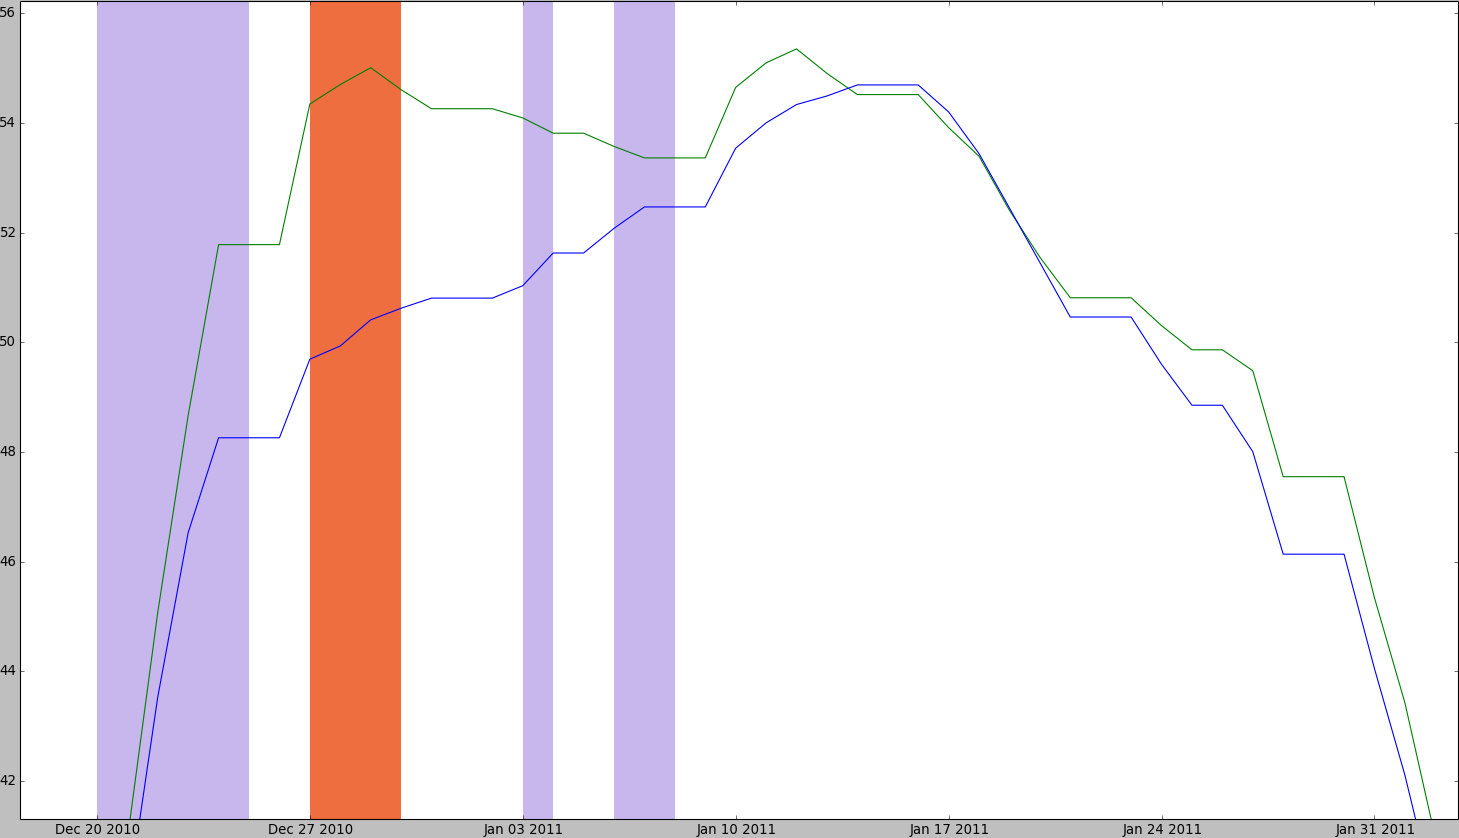
\includegraphics[width=0.8\textwidth]{graphs/Mumbai_RetailvsAvg_ill1.png}
	\caption{Case: 27-Dec-2010 to 29-Dec-2010 (Green line - Centre Retail Price, Blue Line - Average Retail Price)}
	\label{fig:Mumbai_RetailvsAvg_ill1}
	\end{figure}
  
  
  Similar is observed for 17-Oct-2013 to 27-Oct-2013. (See Figure \ref{fig:Mumbai_RetailvsAvg_ill2})
	\begin{figure}[H]
	\centering
	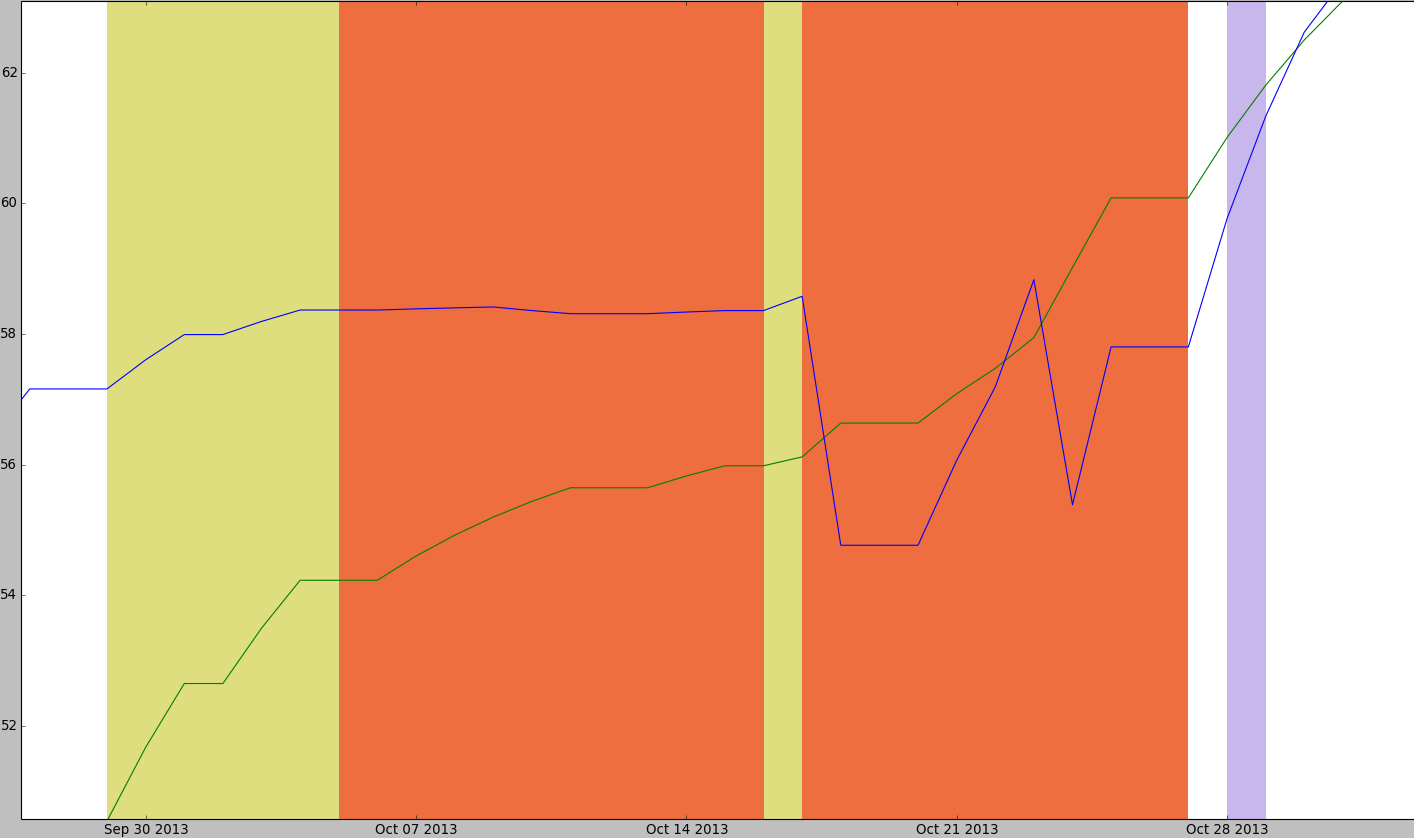
\includegraphics[width=0.8\textwidth]{graphs/Mumbai_RetailvsAvg_ill2.png}
	\caption{Case: 17-Oct-2013 to 27-Oct-2013 (Green line - Centre Retail Price, Blue Line - Average Retail Price)}
	\label{fig:Mumbai_RetailvsAvg_ill2}
	\end{figure}
\item 15-Dec-2010 to 13-Jan-2011 : There was a decrease in the arrival of onion in Mumbai at the start of December which resulted in the increase of retail price. Later arrival seemed nearly constant or increasing but prices continued to grow high. The arrival also increased when the prices were very high which could be the arrival of hoarded stock in market for profiteering.

	\begin{figure}[H]
	\centering
	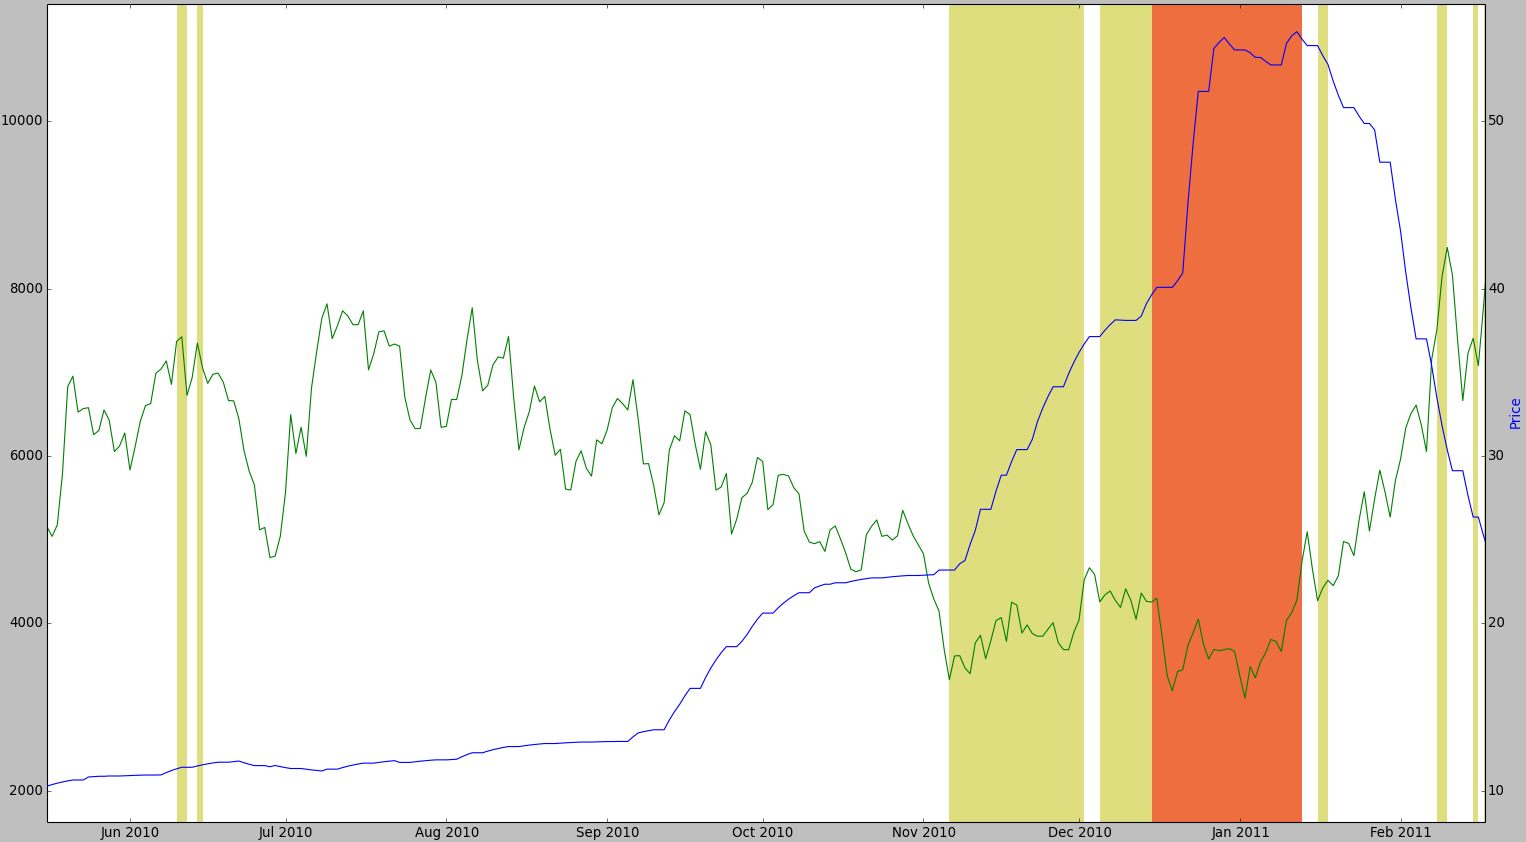
\includegraphics[width=0.8\textwidth]{graphs/Mumbai_RetailvsArrival_ill1.png}
	\caption{Case: 15-Dec-2010 to 13-Jan-2011 (Green line - Arrival Data of Onion, Blue Line - Retail Price)}
	\label{fig:Mumbai_RetailvsArrival_ill1}
	\end{figure}

Similar is observed for 17-Oct-2013 to 25-Nov-2013. (See Figure \ref{fig:Mumbai_RetailvsArrival_ill2})

	\begin{figure}[H]
	\centering
	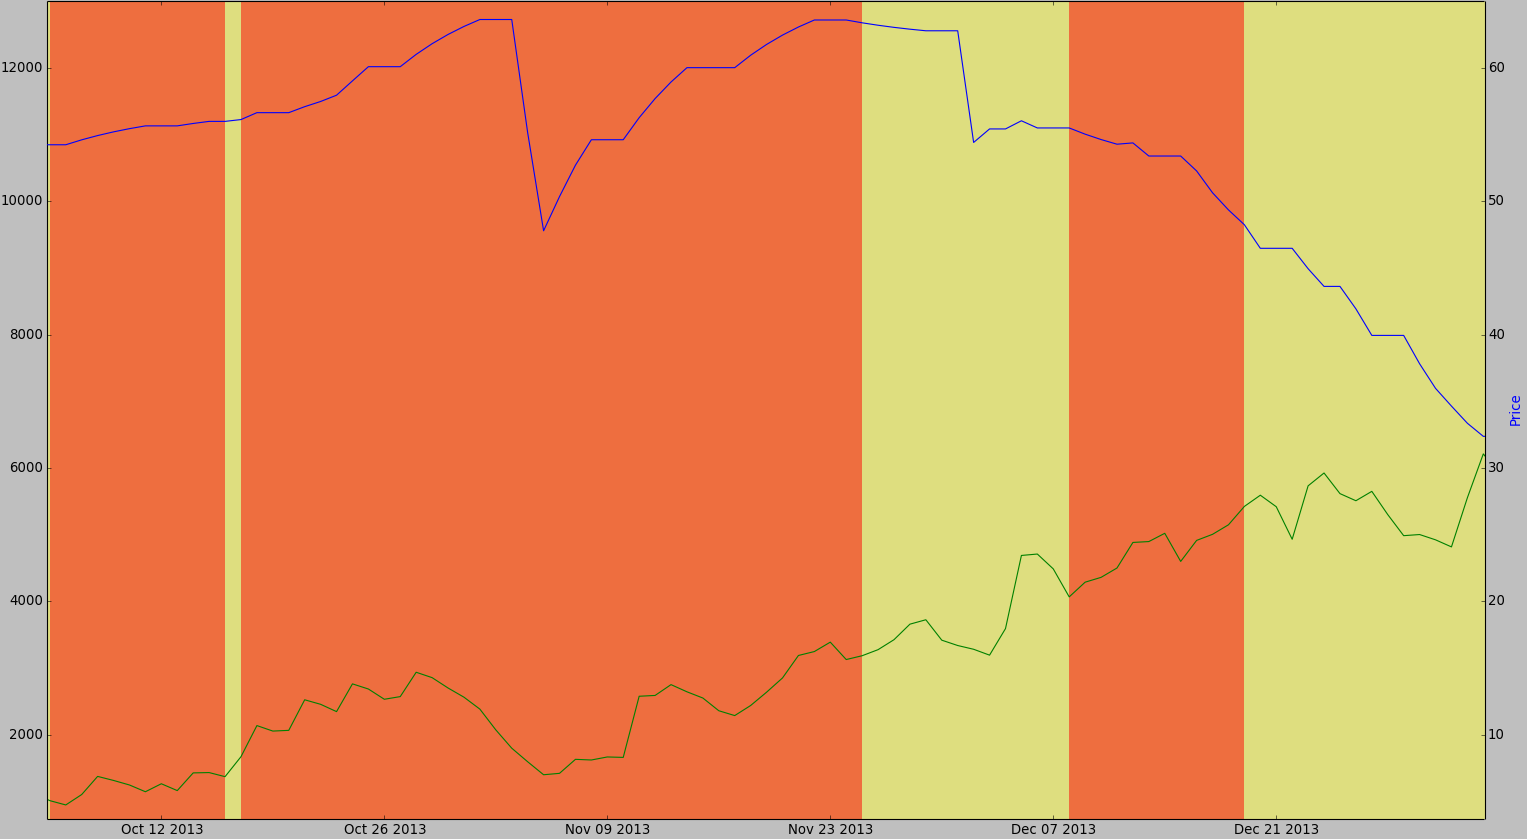
\includegraphics[width=0.8\textwidth]{graphs/Mumbai_RetailvsArrival_ill2.png}
	\caption{Case: 17-Oct-2013 to 25-Nov-2013 (Green line - Arrival Data of Onion, Blue Line - Retail Price)}
	\label{fig:Mumbai_RetailvsArrival_ill2}
	\end{figure}

Similar is observed for 29-Jun-2014 to 06-July-2014 in Delhi. (See Figure \ref{fig:Delhi_RetailvsArrival_ill1})

	\begin{figure}[H]
	\centering
	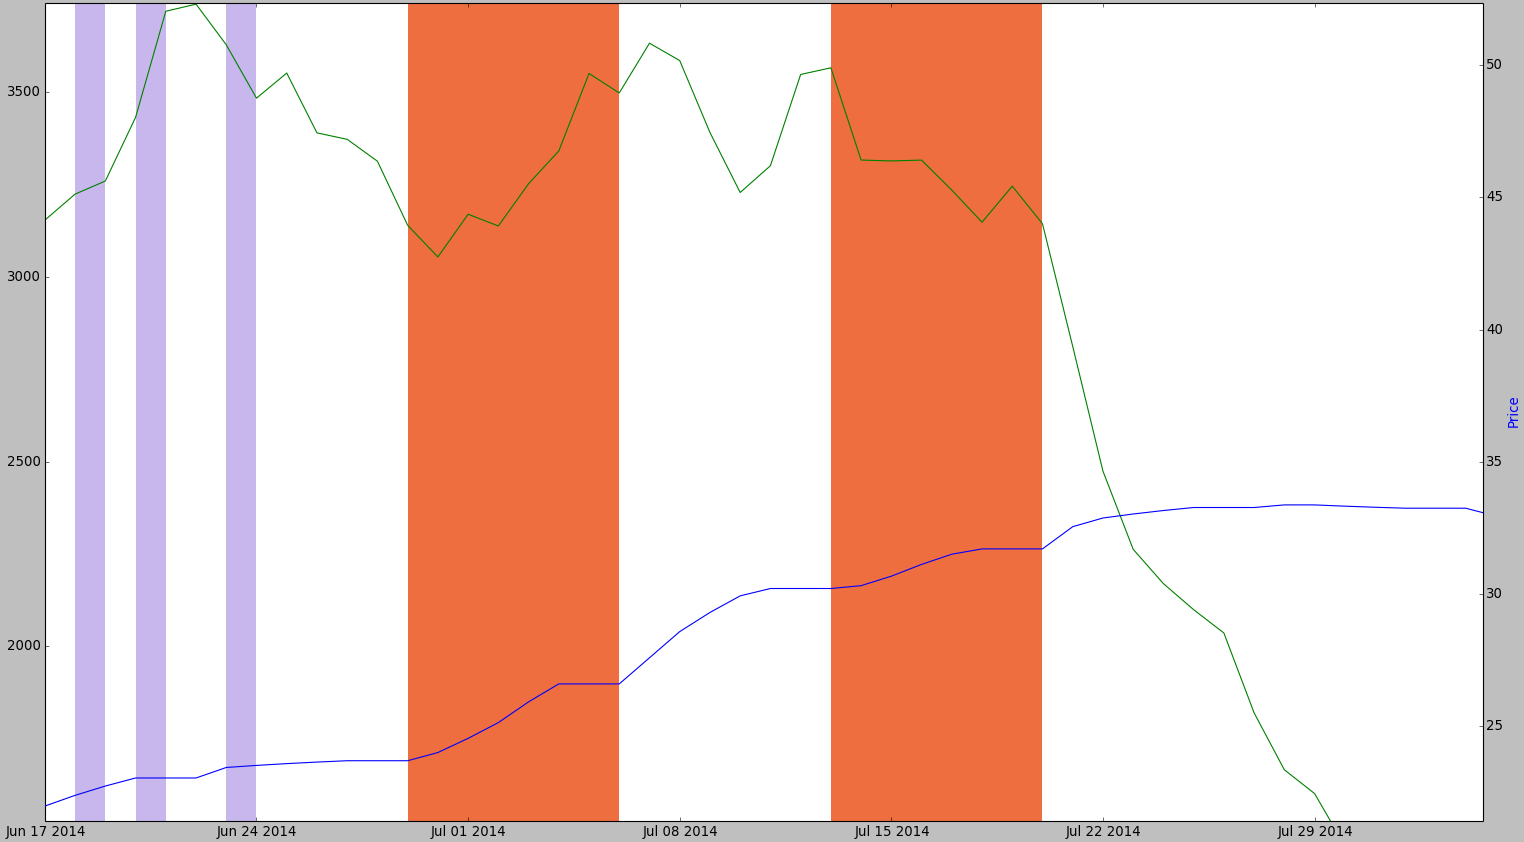
\includegraphics[width=0.8\textwidth]{graphs/Delhi_RetailvsArrival_ill1.png}
	\caption{Case: 29-Jun-2014 to 06-July-2014 (Green line - Arrival Data of Onion, Blue Line - Retail Price)}
	\label{fig:Delhi_RetailvsArrival_ill1}
	\end{figure}

\item 18-Nov-2013 to 24-Nov-2013 : Retail prices are decided by wholesale price. But here in Mumbai, retail price continued to remain high despite of decrease in the wholesale price. (See Figure \ref{fig:Mumbai_RetailvsWS_ill1})

	\begin{figure}[H]
	\centering
	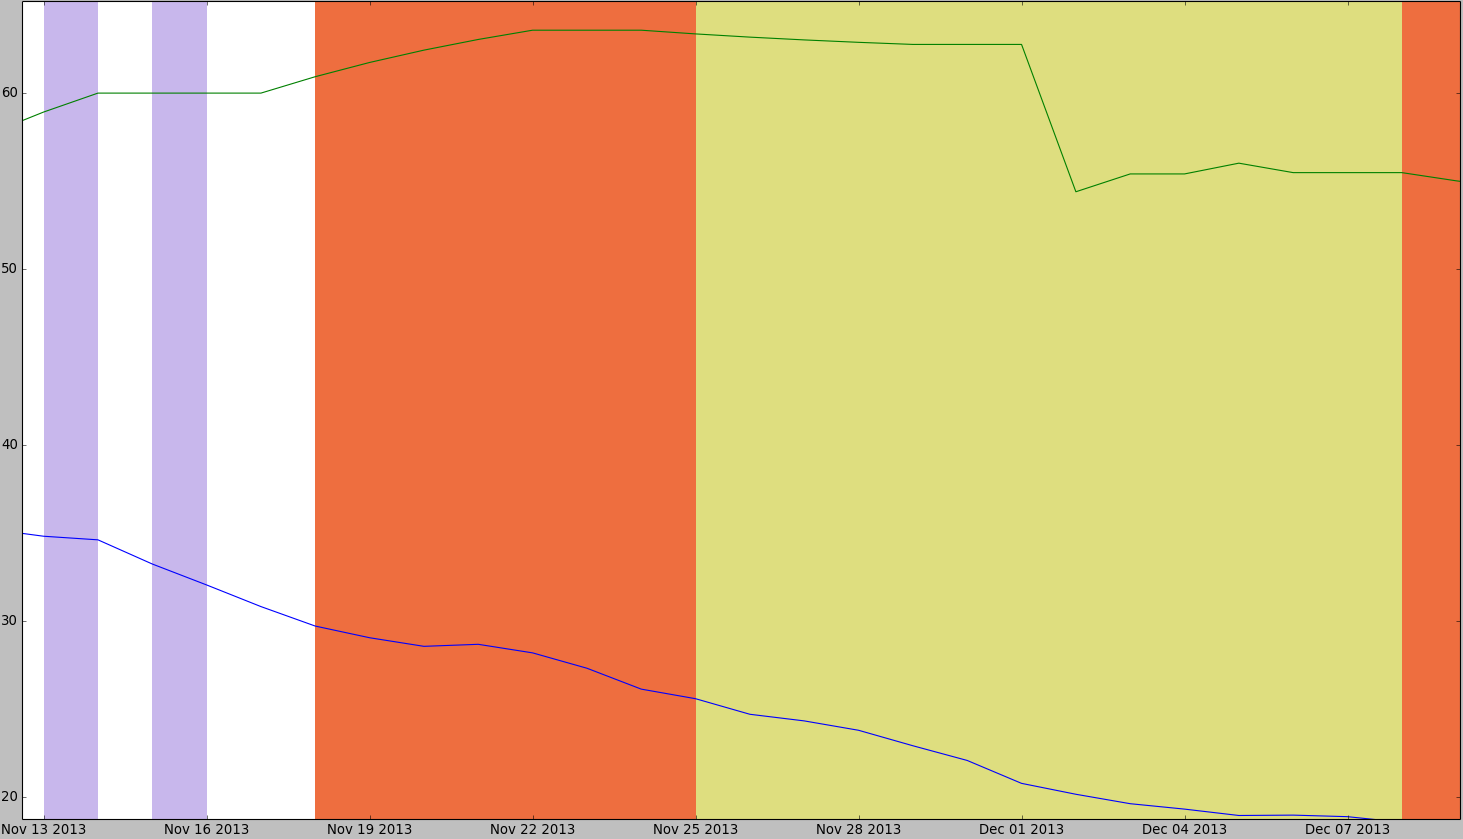
\includegraphics[width=0.8\textwidth]{graphs/Mumbai_RetailvsWS_ill1.png}
	\caption{Case: 18-Nov-2013 to 24-Nov-2013 (Green line - Retail Price, Blue Line - Wholesale Price)}
	\label{fig:Mumbai_RetailvsWS_ill1}
	\end{figure}	
Similar is observed for 21-Oct-2013 to 04-Nov-2013. (See Figure \ref{fig:Mumbai_RetailvsWS_ill2})

	\begin{figure}[H]
	\centering
	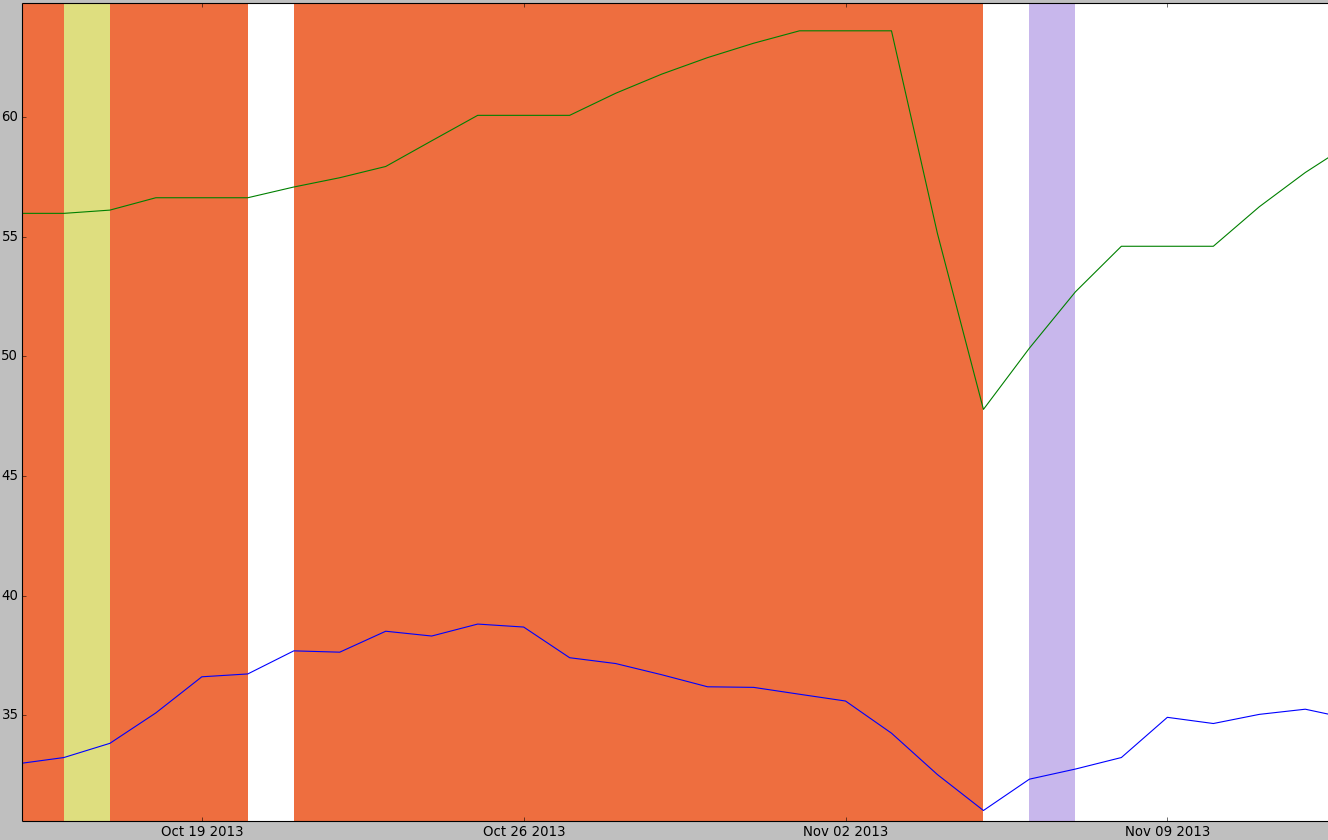
\includegraphics[width=0.8\textwidth]{graphs/Mumbai_RetailvsWS_ill2.png}
	\caption{Case: 21-Oct-2013 to 04-Nov-2013 (Green line - Retail Price, Blue Line - Wholesale Price)}
	\label{fig:Mumbai_RetailvsWS_ill2}
	\end{figure}

Similar is observed for 27-Oct-2013 to 03-Nov-2013 in Delhi. (See Figure \ref{fig:Delhi_RetailvsWS_ill1})

	\begin{figure}[H]
	\centering
	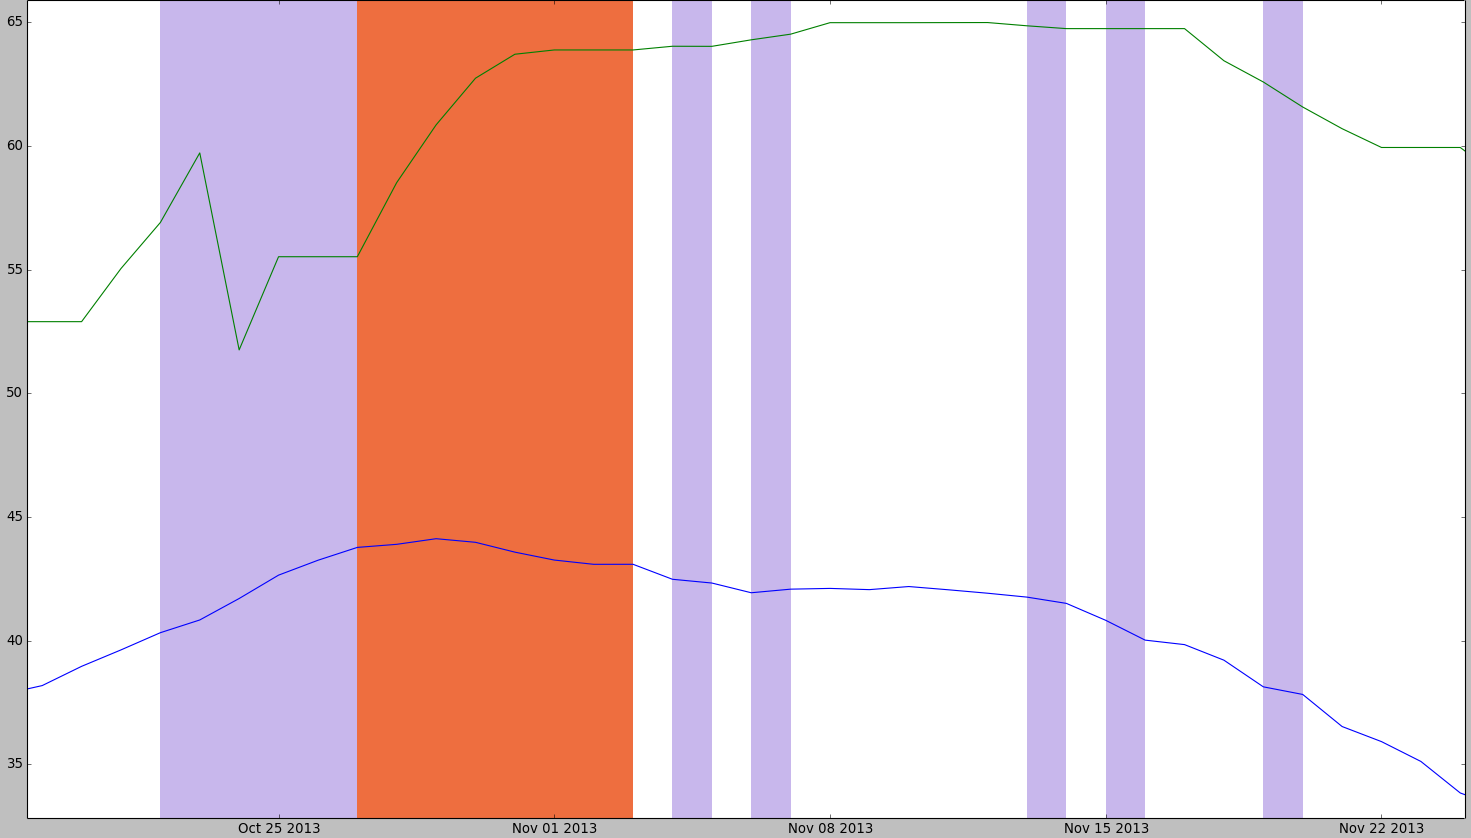
\includegraphics[width=0.8\textwidth]{graphs/Delhi_RetailvsWS_ill1.png}
	\caption{Case: 27-Oct-2013 to 03-Nov-2013 (Green line - Retail Price, Blue Line - Wholesale Price)}
	\label{fig:Delhi_RetailvsWS_ill1}
	\end{figure}

\item 17-Oct-2013 to 24-Nov-2013 : Market observed increase in the arrival on increase of wholesale in Mumbai. The supply crunch could be man-made which resulted in increase in wholesale price and then to take advantage of increased prices, stocks were released in market. (See Figure \ref{fig:Mumbai_WSvsArrival_ill1})
      \begin{figure}[H]
      \centering
      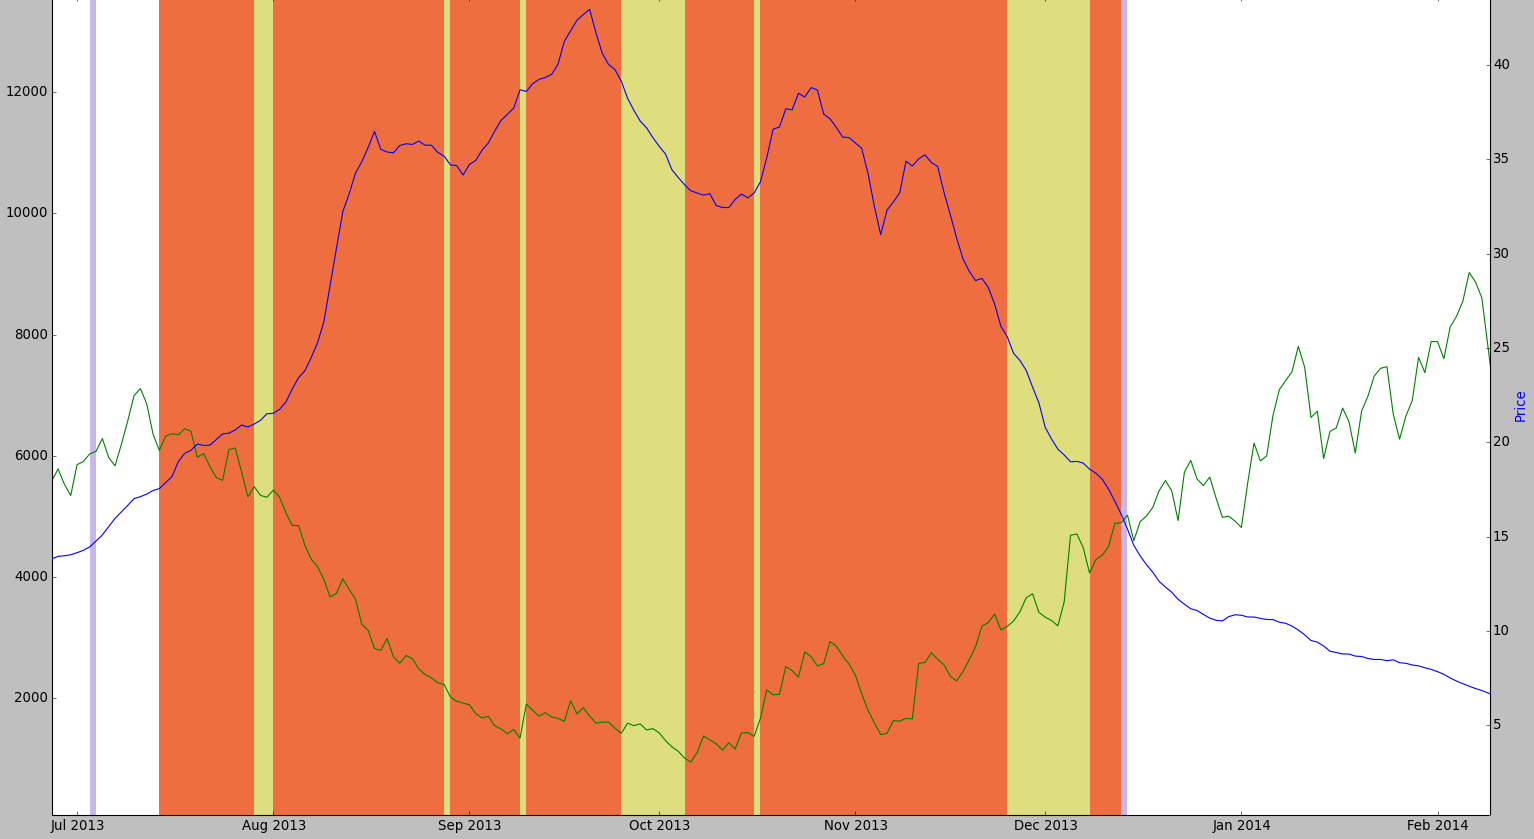
\includegraphics[width=0.8\textwidth]{graphs/Mumbai_WSvsArrival_ill1.png}
      \caption{Case : 17-Oct-2013 to 24-Nov-2013 (Green line - Arrival Data of Onion, Blue Line - Wholesale Price)}
      \label{fig:Mumbai_WSvsArrival_ill1}
      \end{figure}
Similar is observed for 15-Dec-2010 to 12-Jan-2011. (See Figure \ref{fig:Mumbai_WSvsArrival_ill2})
      \begin{figure}[H]
      \centering
      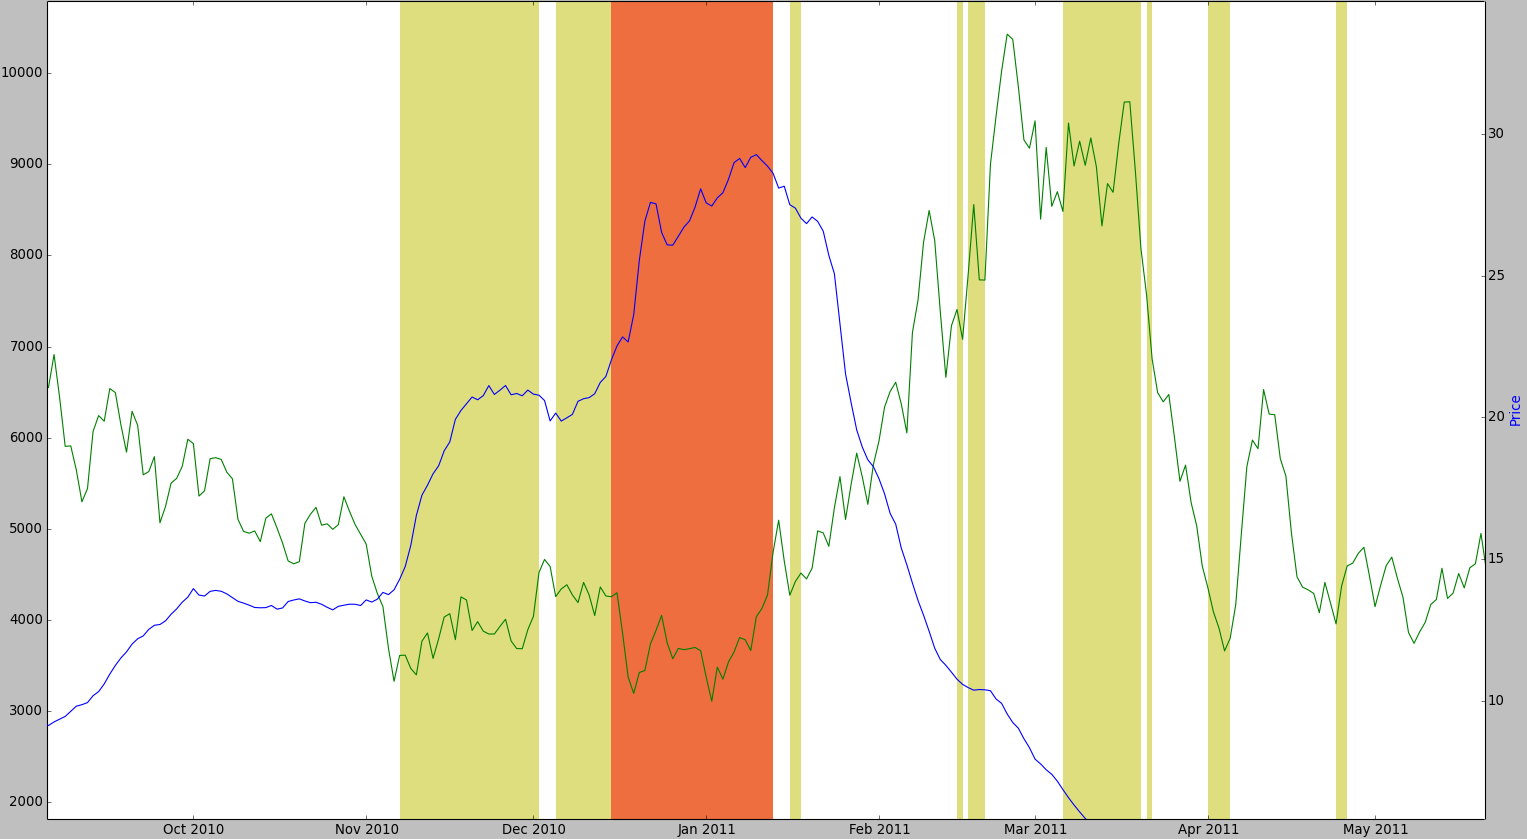
\includegraphics[width=0.8\textwidth]{graphs/Mumbai_WSvsArrival_ill2.png}
      \caption{Case : 15-Dec-2010 to 12-Jan-2011 (Green line - Arrival Data of Onion, Blue Line - Wholesale Price)}
      \label{fig:Mumbai_WSvsArrival_ill2}
      \end{figure}
Similar is observed for 29-Jun-2014 to 05-July-2014 in Delhi. (See Figure \ref{fig:Delhi_WSvsArrival_ill1})
      \begin{figure}[H]
      \centering
      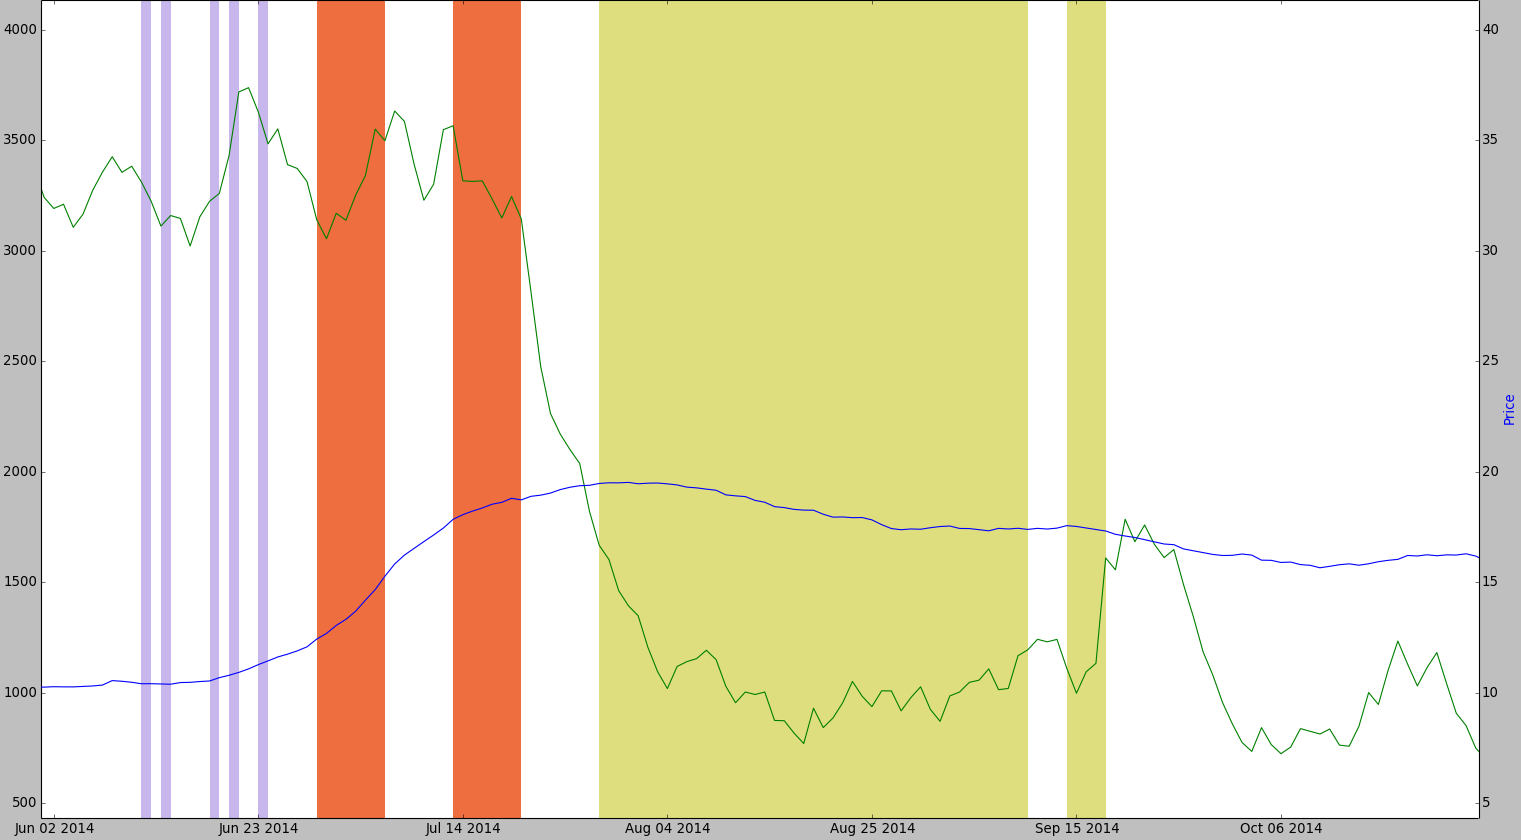
\includegraphics[width=0.8\textwidth]{graphs/Delhi_WSvsArrival_ill1.png}
      \caption{Case : 29-Jun-2014 to 05-July-2014 (Green line - Arrival Data of Onion, Blue Line - Wholesale Price)}
      \label{fig:Delhi_WSvsArrival_ill1}
      \end{figure}
\end{itemize}

\subsubsection{Local News Article Matched Anomaly}
Few of the analysis which were local to center could not be matched with national news articles, but on digging more in regional news article, we could justify the anomaly. One of such case is the anomaly reported on 7th and 8th January 2013, in Delhi, for which news was reported in \href{http://www.jagran.com/news/business-onion-price-affected-from-fog-9987751.html}{Jagran local news paper} on 28th December 2012 which says due to fog there was disruption in the supply of onions. Despite of the speculation on low arrival of onion we observed considerable hike in arrival (which could be hoarded onion stocks brought into market) to earn better profits to take advantage of increased price of onion. Also, we have observed 2 news articles suspecting traders' nexus as the reason for the increased onion prices.


			\begin{figure}[H]
		    	\centering
  		    	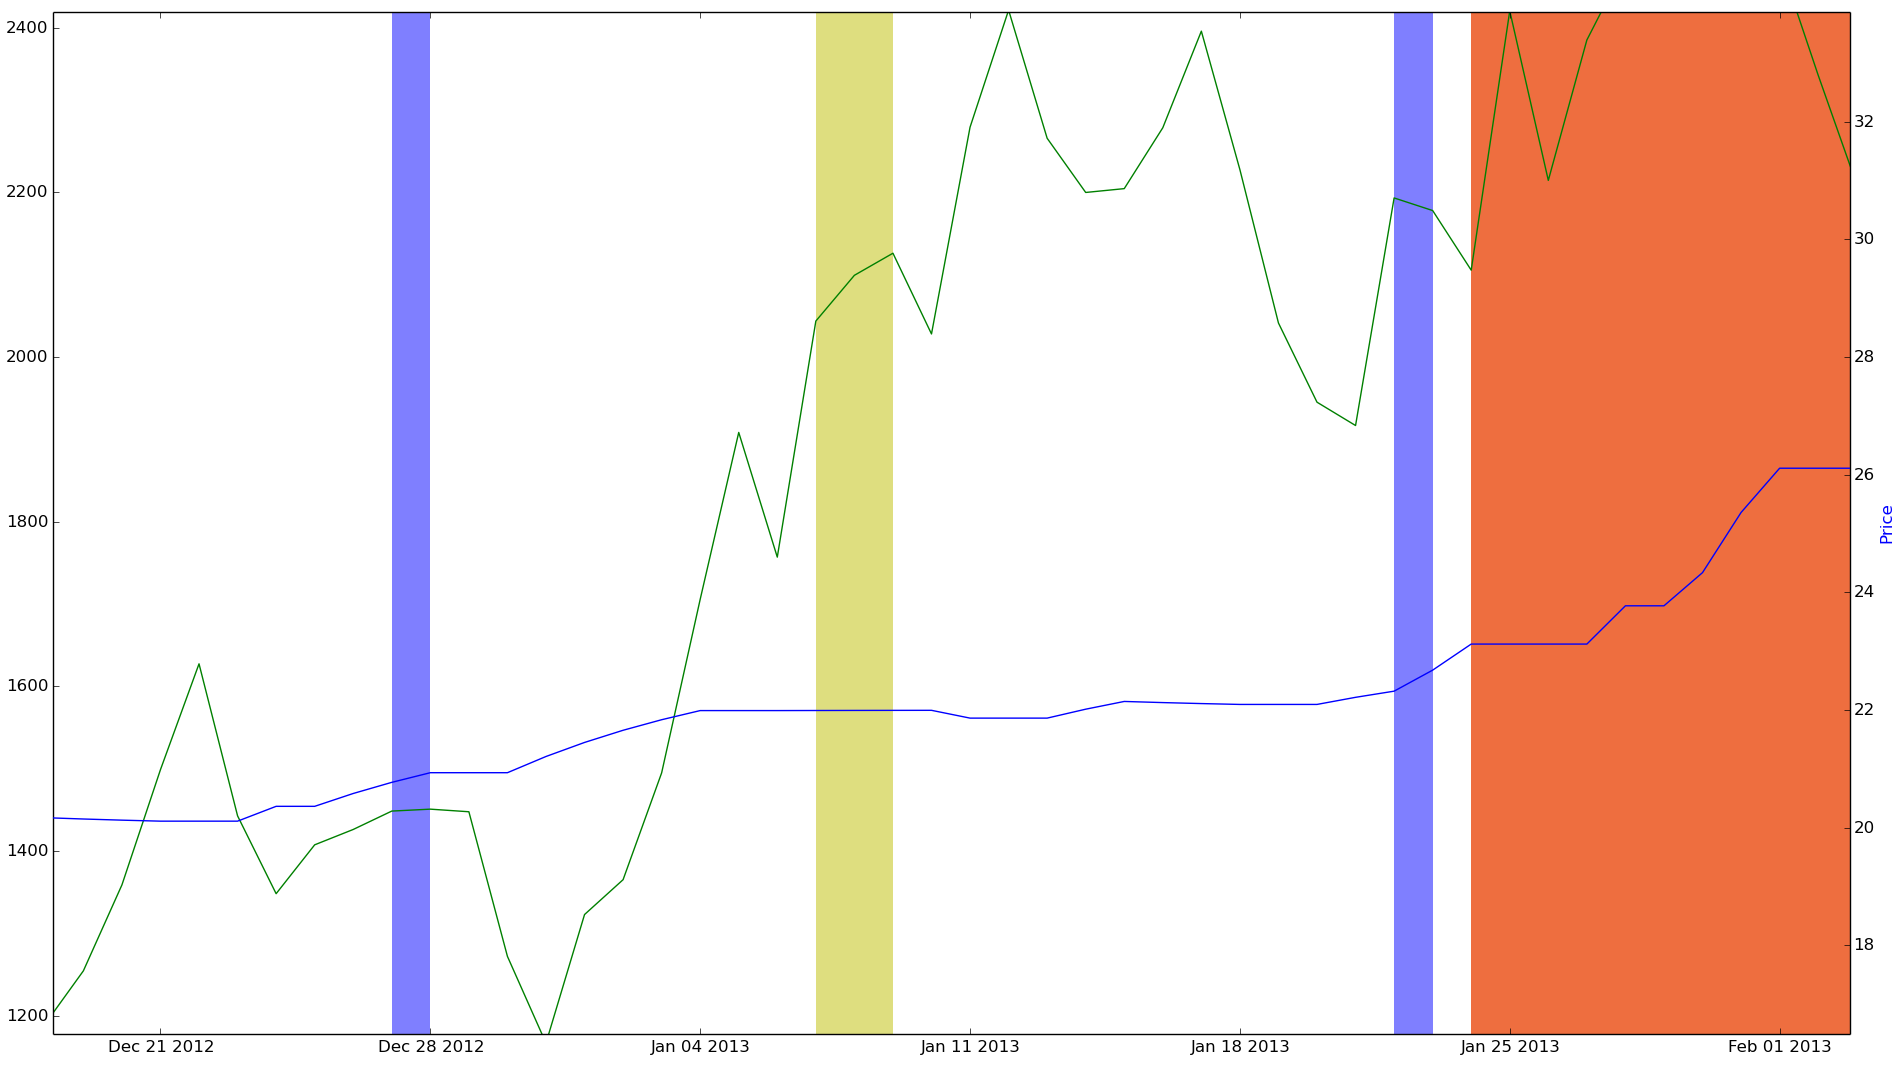
\includegraphics[width=1.1\textwidth]{graphs/localDelhiRegionalNewsPlusNexus.png}
		    	\caption{System Result (Green line - Arrival Data of Onion, Blue Line - Retail Price)}
		    	\label{fig:localExample}
			\end{figure}
			
News Article stated the following,

		\begin{figure}[H]
		    	\centering
  		    	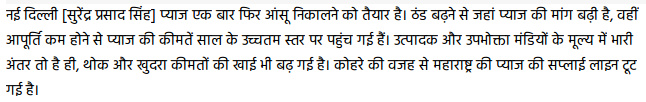
\includegraphics[width=1.1\textwidth]{graphs/localDelhiFog.png}
		    	\caption{Jagran News paper article}
		    	\label{fig:localDelhiFog}
		\end{figure}

\subsubsection{Reported but Not Matched}
Sometimes anomalies are seen even before the news articles actually report them. One of such case is seen in the following figure :
\begin{figure}[H]
\centering
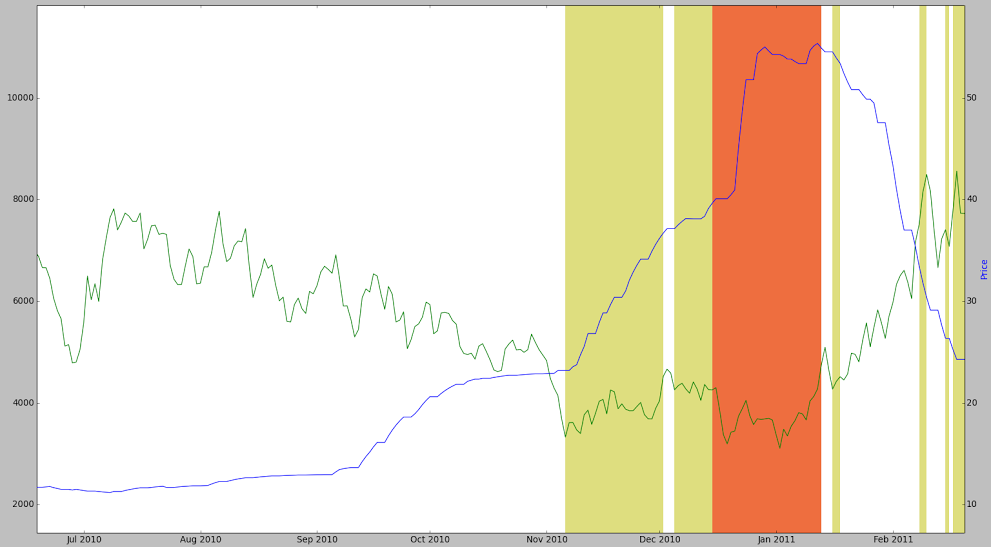
\includegraphics[width=1.1\textwidth]{graphs/ReportedNotMatched.png}
\caption{System Result (Green line - Arrival Data of Onion, Blue Line - Retail Price)}
\label{fig:localExample}
\end{figure}

Here, the anomalies have started being seen in the mid of November. But, the news reported incidents in mid of December. 
\subsubsection{Articles Missed}
In some cases, onion is seen in news because of unseasonal rainfall or low production etc. These cases are not anomalous and rise in prices of onion are expected behaviour. Following is one case, where voilet lines indicate news reported on unseasonal rainfall resulting in low production:

\begin{figure}[H]
\centering
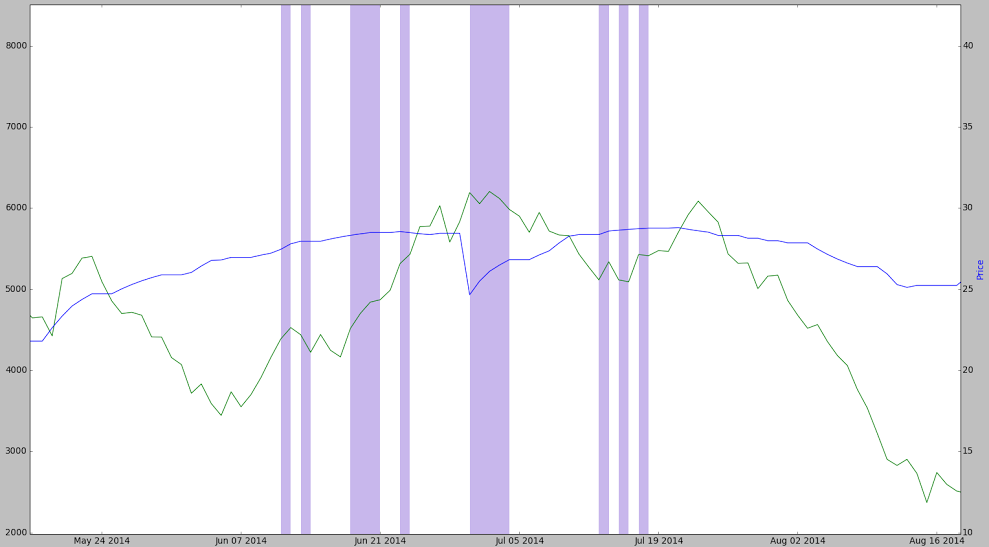
\includegraphics[width=1.1\textwidth]{graphs/MissedAnomaly.png}
\caption{System Result (Green line - Arrival Data of Onion, Blue Line - Retail Price)}
\label{fig:localExample}
\end{figure}

Here, system did not report any anomaly because the arrival has lowered which has lead to the increase in prices which is normal behaviour of system. 

\end{document}   